\pdfinfoomitdate=1
\pdftrailerid{}
\documentclass[11pt]{article}
\usepackage[T1]{fontenc}
\usepackage{lmodern}
\usepackage[a4paper,margin=29mm]{geometry}
\usepackage{amsmath,amssymb,amsthm,mathtools}
\usepackage{microtype}
\usepackage{mathrsfs}
\usepackage{needspace}
\usepackage{booktabs,array,longtable}
\usepackage{enumitem}
\usepackage{xcolor}
\usepackage{tikz}
\usetikzlibrary{arrows.meta,positioning,fit}
\usepackage[hidelinks]{hyperref}
\hypersetup{pdftitle={Global classical solutions of the three-dimensional relativistic Vlasov--Maxwell system},pdfauthor={OpenAI}}
\newcommand{\R}{\mathbb R}
\newcommand{\Id}{\mathrm{Id}}
\DeclareMathOperator{\supp}{supp}
\DeclareMathOperator{\diver}{div}
\DeclareMathOperator{\curl}{curl}
\newtheorem{theorem}{Theorem}[section]
\newtheorem{proposition}[theorem]{Proposition}
\newtheorem{lemma}[theorem]{Lemma}
\newtheorem{corollary}[theorem]{Corollary}
\theoremstyle{definition}
\newtheorem{definition}[theorem]{Definition}
\theoremstyle{remark}
\newtheorem{remark}[theorem]{Remark}
\numberwithin{equation}{section}
\setlength{\emergencystretch}{2em}
\setcounter{tocdepth}{2}
\title{Global classical solutions of the three-dimensional\\relativistic Vlasov--Maxwell system}
\author{OpenAI}
\date{September 23, 2026}
\begin{document}
\maketitle
\begin{abstract}
We prove global existence and uniqueness for arbitrary smooth admissible
initial data in the three-dimensional, one-species relativistic Vlasov--Maxwell
system. The particle density is initially compactly supported, and the
electromagnetic fields have finite energy and bounded derivatives of all orders.
The solution remains smooth on every finite time interval. This resolves the
large-data global classical regularity problem for this model, without size or
symmetry restrictions on the data.
\end{abstract}
\tableofcontents
\section{Introduction}\label{sec:introduction}
The relativistic Vlasov--Maxwell system describes a collisionless plasma
whose particles move under their self-consistent electromagnetic field.
For momentum $v\in\R^3$, write
\[
 q(v)=\sqrt{1+|v|^2},\qquad u(v)=\frac{v}{q(v)}.
\]
The particle density is $f=f(t,x,v)\ge0$; the electric and magnetic fields
are $E=E(t,x)$ and $B=B(t,x)$. We use the one-species normalization
\begin{equation}\label{eq:rvm}
\begin{aligned}
 \partial_t f+u(v)\cdot\nabla_x f+
     (E+u(v)\times B)\cdot\nabla_v f&=0,\\
 \partial_t E-\nabla_x\times B&=-j_f,
 &\partial_t B+\nabla_x\times E&=0,\\
 \nabla_x\cdot E&=\rho_f,
 &\nabla_x\cdot B&=0,
\end{aligned}
\end{equation}
where
\[
 \rho_f(t,x)=\int_{\R^3}f(t,x,v)\,dv,
 \qquad j_f(t,x)=\int_{\R^3}u(v)f(t,x,v)\,dv.
\]
There is no background charge.

A \emph{smooth admissible datum} is a triple $(f_0,E_0,B_0)$ satisfying
\begin{equation}\label{eq:data}
\begin{gathered}
 f_0\in C_c^\infty(\R^3_x\times\R^3_v),\qquad f_0\ge0,\\
 E_0,B_0\in C_b^\infty(\R^3;\R^3)\cap L^2(\R^3;\R^3),\\
 \nabla_x\cdot E_0=\rho_{f_0},\qquad \nabla_x\cdot B_0=0.
\end{gathered}
\end{equation}
Here $C_b^\infty$ means that every spatial derivative is bounded.
A \emph{classical solution} on $[0,T)$ is a $C^1$ triple solving
\eqref{eq:rvm} pointwise, with
$E,B\in C([0,T);L^2_x)$, such that the support of $f$ in $(x,v)$
is contained in a compact set on every compact time subinterval.

\Needspace{12\baselineskip}
\begin{theorem}\label{thm:global}
Every smooth admissible datum \eqref{eq:data} generates a unique global
classical solution of \eqref{eq:rvm}. For every finite $T$, this solution
satisfies
\[
 f\in C^\infty([0,T]\times\R^3_x\times\R^3_v),\qquad
 E,B\in C^\infty([0,T]\times\R^3_x;\R^3),
\]
and $f$ has compact phase-space support on $[0,T]$.
The two divergence constraints hold for all time.
\end{theorem}

Theorem~\ref{thm:global} resolves the large-data global classical
regularity problem for this one-species model in three spatial and three momentum
dimensions. The data have no size or symmetry restriction. The field
assumptions allow a nonzero total charge and its Coulomb tail;
they do not require square-integrability of all field derivatives.
The momentum support bound is on each finite time interval and may
grow with that interval.

\subsection{Historical context}
The distinction between weak existence and classical regularity has
shaped the Cauchy problem for Vlasov--Maxwell. Wollman established local
existence and uniqueness for classical solutions~\cite{Wollman1984}.
DiPerna and Lions developed global weak existence for large
data~\cite{DiPernaLions1989}; a direct formulation for the relativistic
one-species system is given by Rein~\cite{Rein2004Weak}.
These weak existence results do not furnish the regularity and
uniqueness asserted in Theorem~\ref{thm:global}.

For classical solutions, Glassey and Strauss identified bounded
momentum support as a continuation condition~\cite{GlasseyStrauss1986}
and proved global existence for initially dilute
plasmas~\cite{GlasseyStrauss1987}.
Global classical existence was also established by Glassey and
Schaeffer in dimensional reductions: one and one-half dimensions,
two and one-half dimensions, and the planar
problem~\cite{GlasseySchaeffer1990OneHalf,GlasseySchaeffer1997TwoHalf,
GlasseySchaeffer1998PlanarI,GlasseySchaeffer1998PlanarII}.
For the spherically symmetric electrostatic reduction, Glassey and
Schaeffer proved global classical existence for the repulsive relativistic
Vlasov--Poisson system~\cite{GlasseySchaeffer1985Symmetric}.
Rein proved persistence of global existence under small perturbations
of suitably decaying global reference solutions, including nearly
symmetric configurations~\cite{Rein1990Generic}.
These results use restrictions on size, dimension, or the reference
configuration.

The continuation theory also led to new methods. Klainerman and
Staffilani gave a Fourier-based proof of the bounded-momentum
criterion~\cite{KlainermanStaffilani2002}, while Bouchut, Golse and
Pallard gave a physical-space proof using a division lemma for wave
kernels~\cite{BouchutGolsePallard2003}. Luk and Strain showed that it
suffices to control the momentum support after projection onto a
fixed two-dimensional plane~\cite[Theorem~1.2]{LukStrain2014Continuation}.
Moment and spatial-density conditions for continuation were developed by
Pallard~\cite{Pallard2005,Pallard2015Refined}, Sospedra--Alfonso and
Illner~\cite{SospedraAlfonsoIllner2010}, and Luk and
Strain~\cite{LukStrain2016Moments}.
We use the Glassey--Strauss criterion as stated in Luk and
Strain~\cite[Theorem~1.1]{LukStrain2014Continuation};
Section~\ref{cont:continuation} verifies its hypotheses for the
normalization and initial field class considered here.

Small-data theory also developed beyond compact momentum support.
Schaeffer allowed a rapidly decaying momentum tail, retaining compact
spatial support and a suitable smallness
condition~\cite{Schaeffer2004}.
Using a vector-field method with modified commutators, Bigorgne obtained
global existence and sharp asymptotic estimates under weighted smallness
assumptions~\cite{Bigorgne2020}.
His result permits nonzero charge and noncompact particle data.
Wang proved a small-data result without compact support using vector-field
and Fourier methods~\cite{Wang2022SmallData}.
Wei and Yang allow arbitrarily large Maxwell fields with suitable
spatial decay while requiring a sufficiently small weighted particle
density~\cite{WeiYang2021}. Bigorgne subsequently proved global
existence and modified scattering with a small distribution function
and a large Maxwell field~\cite{Bigorgne2025SmallDistribution}.
These theorems preserve a particle-smallness hypothesis.
By prescribing asymptotic data and choosing a sufficiently late starting
time, Bigorgne also constructs particular global solutions with large
particle and field norms~\cite{Bigorgne2023ScatteringMap}. This
construction does not prescribe arbitrary Cauchy data.

Wang's July 2026 two-paper treatment establishes global existence for
large cylindrically symmetric data~\cite{Wang2026I,Wang2026II}.
The first paper develops an iterative smoothing construction and the
second supplies pointwise estimates. Their Theorem~1.1 assumes
$H^s$ fields, $s\ge6$, a weighted $H^s$ particle density, and covariance
of the data under rotations about a fixed axis. It allows localized
noncompact particle data and has no smallness requirement.
The theorem here instead concerns arbitrary compatible compactly
supported particle data, without symmetry, and fields in the class
\eqref{eq:data}. Thus the two data classes should not be identified.

The formulas used below have several classical antecedents.
The retarded-field representation goes back to Glassey and Strauss
\cite{GlasseyStrauss1986}. Luk and Strain organize its most singular
terms using electromagnetic components controlled by energy flux
through light cones~\cite[Proposition~2.2 and Section~3]{LukStrain2014Continuation};
Pallard also uses the orthogonality of the acceleration kernel to the
cone's spatial normal~\cite[Lemma~2.1 and Section~2.3]{Pallard2015Refined}.
The change from retarded phase points to initial particle labels appears
in Lazarovici~\cite[Lemma~9.2]{Lazarovici2016}.
The moving-characteristic cone change of variables is used by Pallard
\cite{Pallard2005}; its proof is also given by Luk and Strain
\cite[Proposition~5.2]{LukStrain2014Continuation}.
We derive the required formulas in the normalization~\eqref{eq:rvm}.

\subsection{Proof strategy}
The central estimate concerns the \emph{signed} change of a particle's
momentum. Along a characteristic $(X(t),V_X(t))$, with
$X'=u(V_X)$ and $V_X'=E(t,X)+u(V_X)\times B(t,X)$, it is the impulse
\[
 V_X(t_2)-V_X(t_1)
 =\int_{t_1}^{t_2}
   \bigl(E(t,X(t))+u(V_X(t))\times B(t,X(t))\bigr)\,dt.
\]
We take the norm after integration. Section~\ref{sec:setup} states the
estimate precisely and shows that it places a lower bound on the time
needed to double the largest particle momentum. These lower bounds have
a divergent sum, which rules out unbounded momentum support in finite
time and allows the continuation criterion to apply.

To estimate the impulse, we follow source particles to their intersections
with the backward light cone of the particle receiving the force.
We divide the source contribution into ranges of momentum, distance, and
angles between the source velocity, receiver velocity, and light ray.
Energy flux through the cone and bounds on the time that source particles
spend in these ranges give the direct force estimates of
Sections~\ref{occ:section} and~\ref{sec:direct}.
At receiver energy comparable to $w$, the absolute-force bound has an
extra factor $\sqrt w$ compared with the signed estimate we need.
The loss occurs when the source velocity is much closer to the light-ray
direction than the receiver velocity is.

In this narrow angular region, we integrate the retarded force along a
source trajectory before taking absolute values.
The identity in Section~\ref{can:section} combines the part without
source acceleration with the part containing it.
The former cancels a term generated by differentiating the cone geometry.
The force is thereby written as a total derivative plus less singular
bulk terms, one of which contains the receiver's acceleration. Expressing
that acceleration through $V_X'$ turns this into an error proportional
to the receiver force. The proof must control its coefficient as well
as the other integration-by-parts errors.

We use the signed identity twice, under an assumed bound on all signed
momentum increments. First, after projection perpendicular to a particle's
momentum, it bounds the number of direction changes of a prescribed
angular size.
This step uses only the preliminary occupation and direct force estimates.
When both source and receiver momenta are large, direction control gives
a stronger occupation bound at intermediate relative angles: between
changes of direction, relative motion makes a monotone crossing of the
region contributing to a fixed range.
Section~\ref{ang:section} proves the direction bound before using it to
improve occupation.

For the second use, Section~\ref{sel:section} selects only those ranges
whose direct force estimates exceed a summable threshold. The other
ranges already satisfy the required bound. On the selected ranges, the
coefficient multiplying the receiver force is at most a constant times
$w^{-1/2}$ after summation. This exactly compensates for the $\sqrt w$
loss in the available absolute-force bound. The occupation improvement
need only hold in the stated angular window: the selection inequalities
force any possible obstruction to this coefficient bound into that
window, where improved occupation rules it out. This yields an impulse
estimate with a time weight that vanishes at the interval endpoints.
Section~\ref{sec:closure}
restores the short endpoint intervals using the assumed signed bound,
obtains a strict improvement, and closes the bootstrap by continuity.

\subsection{Organization}
Section~\ref{sec:setup} states the signed estimate and deduces
Theorem~\ref{thm:global} from it and a continuation result.
Sections~\ref{ret:section}--\ref{sec:direct} derive the retarded force,
occupation estimates and direct bounds.
Section~\ref{can:section} proves the signed cancellation;
Section~\ref{ang:section} bounds direction changes and improves occupation.
Section~\ref{sel:section} estimates the selected signed force, and
Section~\ref{sec:closure} closes the bootstrap.
Section~\ref{sec:continuation-proof} proves local existence, uniqueness,
smooth persistence and the field modification needed to apply the bounded-momentum
continuation theorem to \eqref{eq:data}.

\section{The signed momentum estimate and its consequence}\label{sec:setup}
Our analytic goal is an estimate on momentum increments along
characteristics. We state it first and explain why its logarithmic time
scale excludes finite-time breakdown. Its proof occupies the central
sections of the paper.

Fix a finite horizon $T_0>0$ and a compact interval
$[0,t_*]\subset[0,T_{\max})$, with $t_*\le T_0$, of a classical solution.
A characteristic with initial label $z=(y_{\rm in},v_{\rm in})$ solves
\[
 Y'(s,z)=u(V(s,z)),\qquad
 V'(s,z)=E(s,Y(s,z))+u(V(s,z))\times B(s,Y(s,z)).
\]
It is \emph{supported} if $z\in\supp f_0$.
A distinguished supported characteristic, along which we estimate the
force, is written $(X(t),V_X(t))$ and called the \emph{receiver}.
We write
\[
 a(t)=u(V_X(t)),\quad q_X(t)=q(V_X(t)),\quad K(t)=V_X'(t).
\]
The signed increment is the vector impulse
\[
 V_X(t_2)-V_X(t_1)=\int_{t_1}^{t_2}K(t)\,dt.
\]
Source characteristics continue to use the letters $Y,V,u$.

For nonempty $\supp f_0$, choose a dyadic number $P$ such that
\begin{equation}\label{eq:P-range}
 P\ge1024\max_{\substack{0\le t\le t_*\\z\in\supp f_0}}q(V(t,z)),
 \qquad L=\log(2+P),\qquad S(w)=\frac{P^2L}{w}.
\end{equation}
A dyadic number is a power of two. Receiver scales are $w=2^k$, $k\ge0$.
In every nonempty range $w/8\le q_X\le8w$ one has $w\le P$.

\begin{proposition}[Signed momentum increments]\label{prop:increment}
For each smooth admissible datum and finite $T_0$, there are constants
$M,A\ge1$ and $P_0$ with the following property. On every compact
classical solution interval $[0,t_*]$ as above, for every dyadic
$P\ge P_0$ satisfying \eqref{eq:P-range}, every supported receiver,
every $w=2^k$, $k\ge0$, and every interval $[t_1,t_2]\subset[0,t_*]$
on which $w/8\le q_X(t)\le8w$ throughout, one has
\begin{equation}\label{eq:bootstrap}
 |V_X(t_2)-V_X(t_1)|
 \le MP\sqrt{t_2-t_1}+A(t_2-t_1)S(w).
\end{equation}
The constants are independent of $t_*$ and $P$.
\end{proposition}

\begin{proposition}[Local theory and continuation]\label{prop:continuation}
Every smooth admissible datum has a unique maximal classical solution.
It is smooth on each compact subinterval of its lifespan. If its
maximal time $T_{\max}$ is finite and
\[
 \sup\{\,|v|:0\le t<T_{\max},\ (x,v)\in\supp f(t)\,\}<\infty,
\]
then the solution has a classical extension beyond $T_{\max}$.
\end{proposition}

The proof is given in the final section. It combines the Glassey--Strauss
bounded-momentum criterion in the $H^5$ formulation quoted by Luk and
Strain~\cite[Theorem~1.1 and Footnote~1, arXiv version]{LukStrain2014Continuation}
with a finite-horizon modification of the initial fields. The modification retains the initial Coulomb field
and cuts off vector potentials for the divergence-free remainders.
The removed part evolves as a vacuum Maxwell field that vanishes
throughout the particle region for the chosen horizon. This supplies
Sobolev field data for the continuation theorem while preserving
the original particle dynamics.

\begin{proof}[Proof of Theorem~\ref{thm:global} from
Propositions~\ref{prop:increment} and~\ref{prop:continuation}]
If $f_0=0$, the vacuum Maxwell solution is global and smooth, as shown
in the final section. Suppose $\supp f_0\ne\varnothing$ and, toward a
contradiction, $T_{\max}<\infty$. Proposition~\ref{prop:continuation}
then forces unbounded momentum support. Set $T_0=T_{\max}$ and
\[
 Q(t)=\max_{z\in\supp f_0}q(V(t,z)).
\]
Continuity of the characteristic flow and compactness of the label
set make $Q$ continuous. For all sufficiently large integers $n$,
let $t_n<T_{\max}$ be the first time when $Q(t_n)=2^n$.
Choose a label attaining this value. Along that label let $s_n$
be its last time before $t_n$ at energy $2^{n-1}$. Such a time
exists because the initial energy is smaller; moreover
$s_n\ge t_{n-1}$. On $[s_n,t_n]$ the energy lies in
$[2^{n-1},2^n]$.

Apply Proposition~\ref{prop:increment} on the prefix $[0,t_n]$
with $P=1024\cdot2^n$ and $w=2^n$. Since $q$ is $1$-Lipschitz,
writing $\Delta_n=t_n-s_n$ gives
\[
 2^{n-1}\le |V(t_n)-V(s_n)|
 \le 1024M\,2^n\sqrt{\Delta_n}
   +1024^2A\,2^n\Delta_n\log(2+1024\cdot2^n).
\]
At least one term on the right is at least $2^{n-2}$.
Consequently
\[
 t_n-t_{n-1}\ge\Delta_n
 \ge \frac{c}{\log(2+1024\cdot2^n)}
\]
for a fixed $c>0$. The sum of these lower bounds diverges,
contradicting $t_n<T_{\max}$. Thus $T_{\max}=\infty$.
Uniqueness, smoothness and propagation of the constraints follow
from Proposition~\ref{prop:continuation} and its proof.
\end{proof}

To prove Proposition~\ref{prop:increment}, we assume \eqref{eq:bootstrap} for all such
receivers, scales and intervals in $[0,\tau]$, where $\tau\le t_*$,
and derive a uniform strict improvement. Until that improvement is
proved, \eqref{eq:bootstrap} is a bootstrap assumption.
In the estimates, $C$ and the constants implicit in $\lesssim$ or
$\asymp$ may depend on the datum, $T_0$, and fixed decomposition
parameters, but not on $t_*,P,M,A$. Additional dependence is indicated
explicitly. Lower thresholds on $P$ may depend on $M,A$.
The final choices are made in the order: a time-ramp fraction,
then $M$, then $A$, then the threshold on $P$.

For nonnegative estimates we allow integration over any measurable
subset of receiver times in an interval $J\subset[0,\tau]$ of length
at most $I$, provided those times satisfy $w/8\le q_X\le8w$ and
\begin{equation}\label{eq:short-I}
 0<I\le (w/P)^2.
\end{equation}
The number $I$ is an upper bound on length in these estimates.
For the final signed estimate the interval has length exactly $I$
and the receiver stays in the indicated range throughout.
This distinction permits summation over disjoint time pieces without
introducing a new constant for each piece.

Figure~\ref{fig:dependencies} records the conditional dependencies.
We now prove Proposition~\ref{prop:increment}. Energy and timelike
geometry give preliminary bounds on absolute force. Those bounds
lose a factor at large receiver momentum; the subsequent signed
cancellation removes this loss.

\begin{figure}[htbp]
\centering
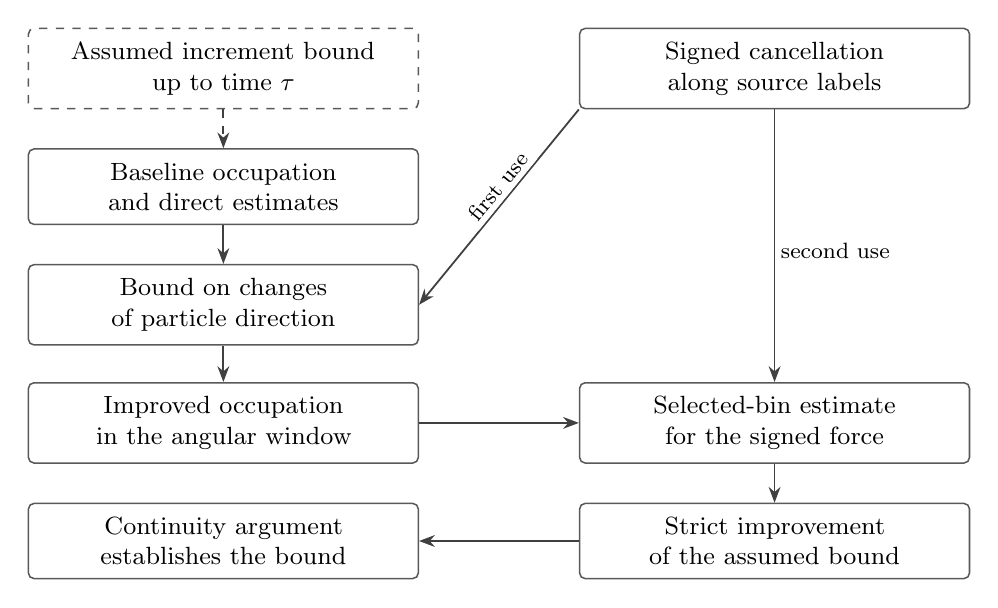
\begin{tikzpicture}[
  x=1cm,y=1cm,
  stage/.style={draw=black!65,rounded corners=2pt,fill=white,
    line width=.55pt,align=center,text width=4.6cm,
    minimum height=.85cm,inner sep=5pt,font=\small},
  flow/.style={-{Stealth[length=2mm]},line width=.65pt,draw=black!75},
  note/.style={font=\footnotesize,fill=white,inner sep=2pt}
]
\node[stage,dashed] (assume) at (0,0)
  {Assumed increment bound\\up to time $\tau$};
\node[stage] (identity) at (7,0)
  {Signed cancellation\\along source labels};
\node[stage] (baseline) at (0,-1.5)
  {Baseline occupation\\and direct estimates};
\node[stage] (direction) at (0,-3)
  {Bound on changes\\of particle direction};
\node[stage] (occupation) at (0,-4.5)
  {Improved occupation\\in the angular window};
\node[stage] (selected) at (7,-4.5)
  {Selected-bin estimate\\for the signed force};
\node[stage] (strict) at (7,-6)
  {Strict improvement\\of the assumed bound};
\node[stage] (close) at (0,-6)
  {Continuity argument\\establishes the bound};
\draw[flow,dashed] (assume) -- (baseline);
\draw[flow] (baseline) -- (direction);
\draw[flow] (identity.south west) --
  node[note,pos=.44,above,sloped] {first use} (direction.east);
\draw[flow] (identity) --
  node[note,pos=.52,right] {second use} (selected);
\draw[flow] (direction) -- (occupation);
\draw[flow] (occupation) -- (selected);
\draw[flow] (selected) -- (strict);
\draw[flow] (strict) -- (close);
\end{tikzpicture}

\caption{Main dependencies in the conditional proof of the signed momentum estimate.
The dashed box is a bootstrap assumption. The first use of signed
cancellation controls particle direction from this assumption and
the baseline estimates; improved occupation is obtained afterward.
The second use yields a strict improvement, and a continuity argument
establishes the initially assumed bound.}
\label{fig:dependencies}

\end{figure}

\section{Energy and the retarded force}\label{ret:section}

The estimates below use the conserved energy and two different changes
of variables on a backward light cone. We first derive the force kernels
without derivatives of the density. This representation belongs to the
Glassey--Strauss approach~\cite{GlasseyStrauss1986}; the organization by
cone-controlled field components also appears in
\cite[Proposition~2.2 and Section~3]{LukStrain2014Continuation}.
We give the source-label calculation explicitly, including its initial
boundary term.

Throughout this section, fix a classical solution on a compact interval
$[0,t_*]$, with $t_*\leq T_0<\infty$, in the class specified in the main
theorem. All limiting operations are justified on this fixed compact
interval. Constants in the final bounds depend only on the initial
data and $T_0$; constants used solely to remove a cutoff may also depend
on the compact-interval momentum support. Retain the characteristic notation fixed in Section~\ref{sec:setup}.

\begin{lemma}[Transport and cone energy]\label{ret:energy}
The characteristic flow preserves phase volume and transports $f_0$.
In particular $0\leq f\leq\|f_0\|_\infty$. Define
\[
 \mathcal U=\frac{|E|^2+|B|^2}{2}+\int qf\,dv,
 \qquad
 \mathcal S=E\times B+\int quf\,dv,
 \qquad
 \mathcal H_0=\int_{\R^3}\mathcal U(0,x)\,dx.
\]
Then
\begin{equation}\label{eq:energy}
 \int_{\R^3}\mathcal U(s,x)\,dx=\mathcal H_0
 \qquad(0\leq s\leq t_*).
\end{equation}
For every vertex $(t,x)$ in this interval, put
$r=t-s$, $y=x-rn$, $n\in S^2$, and
\[
 d=1-n\cdot u(v),\qquad
 G=|E(s,y)+n\times B(s,y)|+|n\cdot B(s,y)|.
\]
Then
\begin{equation}\label{eq:cone-energy}
 \int_0^t\int_{S^2}r^2
 \left(G^2+\int qd f(s,x-rn,v)\,dv\right)dn\,ds
 \leq4\mathcal H_0.
\end{equation}
\end{lemma}

\begin{proof}
The phase vector field has zero divergence: $u$ is independent of $x$,
$E$ is independent of $v$, and
$\nabla_v\cdot(u\times B)=B\cdot(\nabla_v\times\nabla_v q)=0$.
Liouville's formula gives volume preservation, and the Vlasov equation
gives $f(s,Y,V)=f_0(z)$. The flow exists backwards from every finite
phase point on this compact time interval. Indeed, its spatial path
stays in a bounded ball because $|u|<1$; the fields are bounded on the
resulting compact spacetime set, so its momentum cannot escape in
finite time.

Multiplication of Vlasov by $q$ and integration in $v$, followed by
Maxwell's energy identity, give
\[
 \partial_s\mathcal U+\nabla_x\cdot\mathcal S=0,
 \qquad |\mathcal S|\leq\mathcal U.
\]
There is no momentum boundary term because $f$ has compact phase-space
support on the interval. Integrate against spatial cutoffs equal to one
on a ball of radius $R$, with gradient bounded by $C/R$. The error tends
to zero: the fields are bounded in $C([0,t_*];L^2)$ and the particle
energy has compact support and is continuous in time. Passing to the
limit proves conservation.

The outward spatial normal of the ball $|y-x|<t-s$ is $-n$. Its energy
derivative is therefore minus the boundary integral of
$\mathcal U-n\cdot\mathcal S$. At the cone tip the ball energy tends
to zero by local continuity. Hence the exact cone identity is
\[
 \int_0^t\int_{S^2}r^2
   (\mathcal U-n\cdot\mathcal S)(s,x-rn)\,dn\,ds
 =\int_{|y-x|<t}\mathcal U(0,y)\,dy.
\]
Its particle part is $\int qd f\,dv$, and its field part is
\[
 \frac12\bigl(|E+n\times B|^2+|n\cdot B|^2\bigr).
\]
Since $(a+b)^2\leq2(a^2+b^2)$, the last identity implies
\eqref{eq:cone-energy}.
\end{proof}

\subsection{The retarded source labels}

For fixed $t,x$, set $r=|x-y|$, $s=t-r$, and $n=(x-y)/r$ when $r>0$.
The zero-data wave potentials are
\begin{equation}\label{ret:potentials}
 (\Phi,\mathcal A)(t,x)=\frac1{4\pi}
  \int_{|x-y|<t}\int_{\R^3}
       \frac{f(t-|x-y|,y,v)}{|x-y|}(1,u(v))\,dv\,dy.
\end{equation}

The following change to source labels also appears in
\cite[Section~9, Lemma~9.2]{Lazarovici2016}. We give the calculation
for the present flow.

\begin{lemma}[Retarded phase change]\label{ret:phase-change}
Away from the cone tip, the map sending $(y,v)$ at time
$s=t-|x-y|$ to its initial label is one-to-one, with Jacobian
\begin{equation}\label{ret:phase-jacobian}
 dz=d\,dy\,dv,\qquad d=1-n\cdot u(v)>0.
\end{equation}
Its image consists, up to the null set of tip labels, of
\[
 \mathcal L_{t,x}=\{z:|x-Y(0,z)|<t\}.
\]
For such a label, the retarded time solves
\begin{equation}\label{ret:time-equation}
 s+|x-Y(s,z)|=t.
\end{equation}
Consequently \eqref{ret:potentials} equals
\begin{equation}\label{ret:label-potentials}
 (\Phi,\mathcal A)(t,x)=\frac1{4\pi}
       \int_{\mathcal L_{t,x}} f_0(z)\frac{(1,u(V(s,z)))}{rd}\,dz.
\end{equation}
\end{lemma}

\begin{proof}
Let $Z_s$ be the fixed-time inverse phase flow. Its determinant is one
by Lemma~\ref{ret:energy}, and
$\partial_sZ_s=-D Z_s\,(u,V')$. Since $\nabla_y s=n$, the derivative
of $Z_{t-|x-y|}(y,v)$ is the fixed-time derivative multiplied by
\[
 \Id-(u,V')\otimes(n,0).
\]
The determinant of this rank-one perturbation is $1-n\cdot u=d$.

Along a fixed label, the function on the left of
\eqref{ret:time-equation} is strictly increasing. More explicitly,
on any compact part of that characteristic, its increment between
$s_1<s_2$ is at least
$(1-\sup|u|)(s_2-s_1)>0$. It starts below $t$ exactly for labels in
$\mathcal L_{t,x}$ and at $s=t$ is at least $t$. Thus it has exactly
one root. The root is a tip only if $Y(t,z)=x$. This set has phase
Lebesgue measure zero, by the volume-preserving fixed-time flow and
Fubini's theorem. This proves injectivity and the image assertion.
Transport of $f$ and \eqref{ret:phase-jacobian} now give
\eqref{ret:label-potentials}.
\end{proof}

\subsection{The exact electric and magnetic kernels}

Along a source characteristic write
\begin{equation}\label{ret:source-acceleration}
 b=u'=\frac{\Id-u\otimes u}{q}(E+u\times B),
\end{equation}
where these fields, $u$, and $q$ are evaluated at its retarded point.

\begin{proposition}[Retarded field representation]\label{ret:representation}
Let $E^{\rm fr},B^{\rm fr}$ be the homogeneous wave solutions with data
\[
 (E^{\rm fr},\partial_tE^{\rm fr})|_{t=0}
       =(E_0,\nabla\times B_0),\qquad
 (B^{\rm fr},\partial_tB^{\rm fr})|_{t=0}
       =(B_0,-\nabla\times E_0).
\]
For $t>0$, define initial boundary terms by
\begin{equation}\label{ret:initial-boundary}
 \begin{split}
 (E^{\rm bd},B^{\rm bd})(t,x)
 =\frac1{4\pi t}\int_{|x-y_0|=t}\int_{\R^3}
 \frac{f_0(y_0,v_0)}{d_0}
 \bigl(n_0-u_0,\ n_0\times(n_0-u_0)\bigr)\,dv_0\,dS_{y_0},\\
 n_0=(x-y_0)/t,\qquad u_0=u(v_0),\qquad d_0=1-n_0\cdot u_0.
 \end{split}
\end{equation}
Set these terms to zero at $t=0$. Then
\begin{equation}\label{ret:fields}
 \begin{split}
 E(t,x)&=E^{\rm fr}(t,x)+E^{\rm bd}(t,x)
                  +\frac1{4\pi}\int_{\mathcal L_{t,x}}f_0(z)\,\mathscr K\,dz,\\
 B(t,x)&=B^{\rm fr}(t,x)+B^{\rm bd}(t,x)
                  +\frac1{4\pi}\int_{\mathcal L_{t,x}}f_0(z)\,(n\times\mathscr K)\,dz,
 \end{split}
\end{equation}
where
\begin{equation}\label{ret:kernel}
 \mathscr K=\frac{n-u}{r^2q^2d^3}
       +\frac{(n-u)(n\cdot b)-db}{rd^3}.
\end{equation}
All these integrals are well defined at the stated classical regularity.
Moreover,
\begin{equation}\label{ret:data-bound}
 \sup_{0\leq t\leq T_0,\ x\in\R^3}
 (|E^{\rm fr}|+|B^{\rm fr}|+|E^{\rm bd}|+|B^{\rm bd}|)
 \leq C_{T_0,f_0,E_0,B_0}.
\end{equation}
\end{proposition}

\begin{proof}
\emph{Wave representation.}
Kirchhoff's formula gives
$\Box(\Phi,\mathcal A)=(\rho_f,j_f)$ with zero data, where
$\Box=\partial_t^2-\Delta$. Maxwell's equations give, distributionally,
\[
 \Box E=-\nabla\rho_f-\partial_tj_f,\qquad
 \Box B=\nabla\times j_f.
\]
Thus the fields are
$(-\nabla\Phi-\partial_t\mathcal A,\nabla\times\mathcal A)$ plus
the stated homogeneous waves. Here it is important that the electric
potential contribution has initial time derivative $-j_f(0)$.

We justify this assertion with only $C^1$ sources. In the variables
$y=x-rn$, the potentials integrate a $C^1$ source against $r\,dr\,dn$.
Their first derivatives are continuous, and locally uniformly in $x$,
\[
 \partial_t\mathcal A(t,x)=t j_f(0,x)+O(t^2),\qquad
 \nabla\Phi(t,x),\ \nabla\mathcal A(t,x)=O(t^2).
\]
These formulas give the required zero initial values and initial
difference quotients of the potential fields. For completeness,
uniqueness of the resulting continuous distributional wave remainder
can be reduced to classical uniqueness: convolve spatially with a
compact smooth mollifier. The wave equation then supplies a continuous
second time derivative, including at zero; the initial difference
quotients identify its zero initial velocity. Local wave energy gives
zero, and removal of the mollifier gives the assertion. No second
derivative of $f$ is used.

\emph{Interior kernels.}
To differentiate \eqref{ret:label-potentials}, hold the initial label
fixed. Implicit differentiation of \eqref{ret:time-equation} gives
\[
 s_t=1/d,\qquad\nabla_xs=-n/d.
\]
Write $\ell=(rd)^{-1}$. With $s$ held fixed,
\[
 \nabla_x\ell=-\frac{n-u}{r^2d^2}.
\]
With $x$ fixed,
\[
 r_s=-n\cdot u,\qquad
 n_s=-\frac{u-n(n\cdot u)}r,\qquad
 \ell_s=\frac{q^{-2}-d}{r^2d^2}+\frac{n\cdot b}{rd^2}.
\]
Therefore the interior electric kernel is
\[
 -\nabla_x^{\rm total}\ell-\partial_t(u\ell)
 =\frac{n-u}{r^2d^2}+\frac{n-u}{d}\ell_s-\frac b{rd^2},
\]
which simplifies to \eqref{ret:kernel}. In the magnetic curl the
corresponding expression is its cross product with $n$: indeed
\[
 \nabla_x^{\rm total}\times(u\ell)
 =\left(-\frac{n-u}{r^2d^2}-\frac n d \ell_s\right)\times u
                  -\frac{n\times b}{rd^2}
 =n\times\mathscr K.
\]

\emph{Boundary terms and the cone tip.}
The label domain has indicator $\mathbf1_{\{t>|x-y_0|\}}$.
Its time derivative is $\delta(t-|x-y_0|)$ and its spatial gradient is
$-n_0\delta(t-|x-y_0|)$. The resulting electric factor is
$(n_0-u_0)/(td_0)$ and the magnetic one is its cross product with $n_0$.
Integration over the initial sphere gives \eqref{ret:initial-boundary}.
The initial velocities are bounded on $\operatorname{supp}f_0$, so
$d_0$ has a fixed positive lower bound. Sphere area and compact initial
velocity support consequently give
$|E^{\rm bd}|+|B^{\rm bd}|\leq C_{f_0}t$, uniformly in $x$.

The differentiations at the cone tip can be justified by inserting a
smooth cutoff that vanishes for $r<\gamma$ and equals one for
$r>2\gamma$. On the supported labels of the fixed compact time interval,
$d$ is bounded below and $u,b$ are bounded. Derivatives of this cutoff
are at most $C/\gamma$. By \eqref{ret:phase-jacobian}, the omitted
potential and cutoff errors are bounded by integrals of $Cf/r$ over
$r<2\gamma$, multiplied by at most $C/\gamma$ for the latter. They
are $O(\gamma^2)$ and $O(\gamma)$, respectively. The omitted kernel
integrals are $O(\gamma)$ because their worst radial singularity after
this change of variables is $r^{-2}$. These bounds are locally uniform
for $t>0$. The already established initial traces handle $t=0$.
Thus no term supported at the cone tip remains.

Finally, Kirchhoff's formula for a homogeneous wave $W$ with data
$(W_0,W_1)$ bounds it by
\[
 \|W(t)\|_\infty
 \leq\|W_0\|_\infty+t\|\nabla W_0\|_\infty+t\|W_1\|_\infty.
\]
The assumed bounded initial derivatives give \eqref{ret:data-bound}.
The homogeneous waves here need not together be a vacuum Maxwell
solution; the representation requires only their displayed wave data.
\end{proof}

\subsection{Receiver geometry and pointwise force bounds}

Let $(X(t),V_X(t))$ be a supported receiver characteristic and write
\[
 \begin{gathered}
 a=u(V_X),\qquad q_X=q(V_X),\qquad K=V_X',\\
 D=1-n\cdot a,\qquad e=1-a\cdot u,\qquad Q=D\Id+n\otimes a.
 \end{gathered}
\]
Since $h+a\times(n\times h)=Qh$, Proposition~\ref{ret:representation}
and \eqref{ret:phase-jacobian} give
\begin{equation}\label{ret:force}
 K=K^{\rm data}+\frac1{4\pi}\int_{|X(t)-y|<t}\int_{\R^3}
                (T_{\rm ker}+S_{\rm ker})\,dv\,dy,
\end{equation}
where $|K^{\rm data}|\leq C_{T_0,f_0,E_0,B_0}$ and
\begin{equation}\label{ret:force-kernels}
 T_{\rm ker}=\frac{fQ(n-u)}{r^2q^2d^2},\qquad
 S_{\rm ker}=\frac{fQ\bigl((n-u)(n\cdot b)-db\bigr)}{rd^2}.
\end{equation}
The density and source quantities in these integrals are evaluated at
$(t-r,y,v)$, not at the receiver.

Figure~\ref{fig:retarded-geometry} shows the source and receiver geometry.
\begin{figure}[tbp]
  \centering
  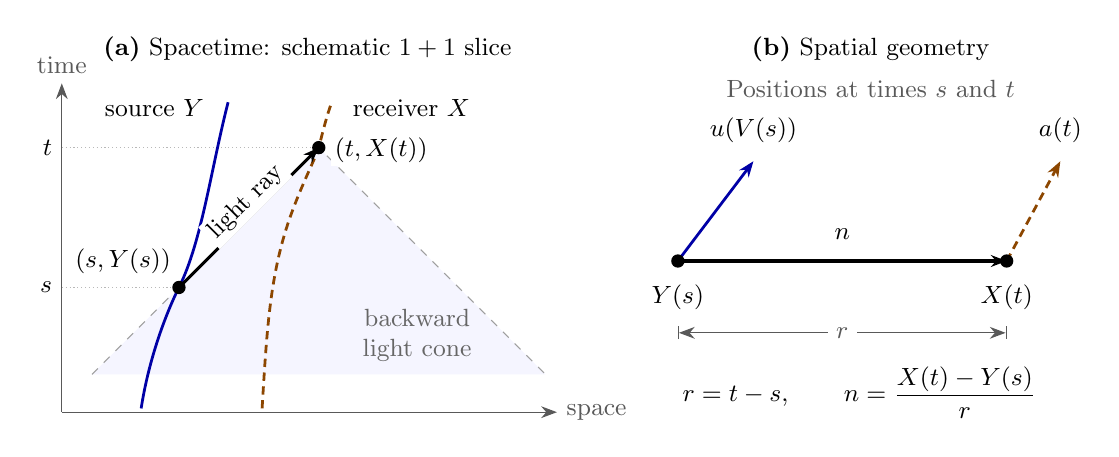
\begin{tikzpicture}[
      x=0.96cm,y=0.96cm,font=\small,
      >={Stealth[length=2mm]},
      source/.style={draw=blue!65!black,line width=1pt},
      receiver/.style={draw=orange!55!black,line width=1pt,densely dashed},
      event/.style={circle,fill=black,inner sep=1.7pt},
      guide/.style={draw=black!28,densely dotted},
      labelbox/.style={fill=white,inner sep=1.5pt}
    ]
    \node at (3.4,5.2) {\textbf{(a)} Spacetime: schematic $1+1$ slice};
    \fill[blue!4] (0.55,0.9)--(3.55,3.9)--(6.55,0.9)--cycle;
    \draw[black!38,dashed] (0.55,0.9)--(3.55,3.9)--(6.55,0.9);
    \draw[->,black!65] (0.15,0.4)--(0.15,4.75) node[above] {time};
    \draw[->,black!65] (0.15,0.4)--(6.7,0.4) node[right] {space};
    \draw[guide] (0.15,2.05)--(1.7,2.05);
    \draw[guide] (0.15,3.9)--(3.55,3.9);
    \node[left] at (0.15,2.05) {$s$};
    \node[left] at (0.15,3.9) {$t$};
    \draw[source] (1.2,0.45)
      .. controls (1.3,1.1) and (1.525,1.7) .. (1.7,2.05)
      .. controls (2.0,2.65) and (2.12,3.6) .. (2.35,4.5);
    \draw[receiver] (2.8,0.45)
      .. controls (2.86,1.45) and (2.9,2.2) .. (3.16,2.95)
      .. controls (3.316,3.4) and (3.525,3.8) .. (3.55,3.9)
      .. controls (3.6075,4.13) and (3.65,4.3) .. (3.72,4.5);
    \node[source,draw=none,anchor=east] at (2.17,4.42) {source $Y$};
    \node[receiver,draw=none,anchor=west] at (3.86,4.42) {receiver $X$};
    \draw[->,line width=1.1pt] (1.7,2.05)--(3.55,3.9);
    \node[event] at (1.7,2.05) {};
    \node[event] at (3.55,3.9) {};
    \node[anchor=south east,inner sep=0pt] at (1.60,2.23) {$(s,Y(s))$};
    \node[labelbox,anchor=west] at (3.7,3.87) {$(t,X(t))$};
    \node[align=center,black!60] at (4.85,1.42) {backward\\light cone};
    \node[labelbox,rotate=45] at (2.58,3.18) {light ray};

    \node at (10.85,5.2) {\textbf{(b)} Spatial geometry};
    \node[black!65] at (10.85,4.68) {Positions at times $s$ and $t$};
    \draw[->,line width=1.1pt] (8.3,2.4)--(12.65,2.4)
      node[midway,above=4pt] {$n$};
    \draw[source,->] (8.3,2.4)--(9.3,3.72)
      node[above=3pt] {$u(V(s))$};
    \draw[receiver,->] (12.65,2.4)--(13.36,3.72)
      node[above=3pt] {$a(t)$};
    \node[event] at (8.3,2.4) {};
    \node[event] at (12.65,2.4) {};
    \node[below=5pt] at (8.3,2.4) {$Y(s)$};
    \node[below=5pt] at (12.65,2.4) {$X(t)$};
    \draw[|<->|,black!65] (8.3,1.45)--(12.65,1.45)
      node[midway,fill=white,inner sep=3pt] {$r$};
    \node at (10.7,0.66) {$\displaystyle
      r=t-s,\qquad n=\frac{X(t)-Y(s)}{r}$};
  \end{tikzpicture}
  \caption{Retarded geometry along a receiver characteristic.
  The source event $(s,Y(s))$ lies on the backward light cone of
  $(t,X(t))$, with $r=t-s=|X(t)-Y(s)|>0$.
  The spatial unit vector $n$ points from $Y(s)$ to $X(t)$.
  Panel~(b) shows the source velocity $u(V(s))=Y'(s)$ and the
  receiver velocity $a(t)=X'(t)$ at these respective events.
  The curves and vector directions are schematic.}
  \label{fig:retarded-geometry}
\end{figure}


\begin{lemma}[Pointwise force bounds]\label{ret:direct-bounds}
Let $\theta,\phi>0$ satisfy $\theta^2\asymp d$ and $\phi^2\asymp D$,
with fixed comparison constants. The transport kernel splits into two
terms, according to the normal and tangential parts of $n-u$, bounded by
\begin{equation}\label{ret:transport-bounds}
 T_r=\frac{Cf}{r^2q^2\theta^2},\qquad
 T_\perp=\frac{Cf\phi}{r^2q^2\theta^3}.
\end{equation}
With $G$ as in Lemma~\ref{ret:energy}, the source acceleration satisfies
\begin{equation}\label{ret:acceleration-bounds}
 |b|\leq\frac Cq(G+\theta^2|B|),\qquad
 |n\cdot b|\leq\frac{C\theta}q(G+\theta^2|B|),\qquad
 |q'|\leq C(G+\theta|B|).
\end{equation}
Consequently
\begin{equation}\label{ret:source-bounds}
 |S_{\rm ker}|\leq S_g+S_b,\qquad
 S_g=\frac{Cf\phi}{rq\theta^2}G,\qquad
 S_b=\frac{Cf\phi}{rq}|B|.
\end{equation}
If $V_X\ne0$ and $P_X$ is orthogonal projection onto $V_X^\perp$, then
$|P_XS_{\rm ker}|\leq C\phi(S_g+S_b)$.
\end{lemma}

\begin{proof}
The exact identities
\[
 2d=|n-u|^2+q^{-2},\qquad
 2D=|n-a|^2+q_X^{-2}
\]
give $|n-u|\leq C\theta$ and $|n-a|\leq C\phi$.
Also $Qn=n$, whereas for $h\perp n$,
\[
 |Qh|\leq D|h|+|a\cdot h|\leq C\phi|h|.
\]
The normal component of $n-u$ is $dn$ and its tangential component has
norm at most $C\theta$. This proves \eqref{ret:transport-bounds}.

Put $u=(1-d)n+u_\perp$ and $H=E+n\times B$. The force at the source is
\[
 F_{\rm src}=E+u\times B=H+(-dn+u_\perp)\times B.
\]
Its tangential and normal components satisfy
\[
 |(F_{\rm src})_\perp|\leq C(G+\theta^2|B|),\qquad
 |n\cdot F_{\rm src}|\leq C(G+\theta|B|).
\]
Indeed the tangential part of $u_\perp\times B$ involves only
$n\cdot B$, while its normal part is bounded by $C\theta|B|$.
For $L_u=\Id-u\otimes u$ we have
\[
 |L_un|\leq C\theta,\qquad
 |n\cdot L_un|=2d-d^2\leq C\theta^2,
 \qquad |n\cdot L_uh|\leq C\theta|h|\quad(h\perp n).
\]
Combining these component bounds with $b=q^{-1}L_uF_{\rm src}$ proves
the first two inequalities in \eqref{ret:acceleration-bounds}.
The last follows from $q'=u\cdot E=u\cdot H-u\cdot(n\times B)$.

The numerator $N=(n-u)(n\cdot b)-db$ is tangent to $n$, since
$n\cdot N=d(n\cdot b)-d(n\cdot b)=0$. This cone tangency is also used
in \cite[Lemma~2.1]{Pallard2015Refined}. The preceding estimates give
\[
 |N|\leq\frac{C\theta^2}{q}(G+\theta^2|B|).
\]
The tangential bound for $Q$ now proves \eqref{ret:source-bounds}.
Finally $P_Xa=0$, so $|P_Xn|=|P_X(n-a)|\leq C\phi$. For $h\perp n$,
\[
 |P_XQh|\leq D|h|+|P_Xn|\,|a\cdot h|
               \leq C\phi^2|h|.
\]
Applying this to $N$ gives the additional projected factor.
\end{proof}

\begin{lemma}[Source time along a receiver]\label{ret:receiver-time}
Along a retarded source label satisfying
$t=s+|X(t)-Y(s,z)|$ away from collisions,
\begin{equation}\label{ret:receiver-jacobians}
 \frac{dt}{ds}=\frac dD,\qquad
 ds\,f_0(z)\,dz=D\,dt\,f(t-r,y,v)\,dy\,dv.
\end{equation}
For $f_0(z)dz$-almost every label there is no same-time collision
$Y(t,z)=X(t)$ anywhere in the compact time interval. Such a label has
one continuously differentiable retarded branch after its initial-cone entry, when that
entry occurs, and $r$ is bounded below on each closed part of this
branch in the compact interval.
\end{lemma}

\begin{proof}
Differentiate $t-s-|X(t)-Y(s,z)|=0$ to obtain $D\,dt=d\,ds$.
Both factors are positive. Combining this with
\eqref{ret:phase-jacobian} gives the measure identity in
\eqref{ret:receiver-jacobians}.

To exclude same-time collisions, let $R_v$ bound the supported momenta
on $[0,t_*]$. Use a time grid of mesh at most $\zeta$ with
$O(1+t_*/\zeta)$ points. If a collision occurs, at a nearest grid time
the two positions are at distance at most $2\zeta$, since both spatial
speeds are at most one. At each grid time the mass of labels satisfying
this distance bound is at most
$C\|f_0\|_\infty R_v^3\zeta^3$, by phase-volume preservation.
The union has mass $O(\zeta^2)$ and tends to zero.

For the remaining labels, strict timelikeness gives uniqueness and
continuous differentiability of the retarded root. The entry time is unique because
$t-|X(t)-Y(0,z)|$ is strictly increasing. At entry $r=t>0$, since
an entry at zero would be an excluded initial collision. On any
closed part of the branch, continuity and the absence of collisions
give a positive minimum of $r$. This assertion is labelwise; no
uniform lower bound over all labels is used.
\end{proof}

\section{Occupation of retarded bins}\label{occ:section}

We estimate how much particle mass a receiver can meet in a prescribed
momentum, angle, and distance range. Two changes of variables give crude
bounds. The signed increment assumption then limits how long a source can
remain close to the receiver. A time-averaged energy budget will make the
result summable over the small angular sector.

The residence-time and relative-velocity viewpoint is inspired by
Pfaffelmoser's Vlasov--Poisson argument \cite{Pfaffelmoser1992}.
This is methodological inspiration, not a theorem input for the
Vlasov--Maxwell system: the retarded geometry and source-acceleration
terms require the estimates proved here.

Throughout this section assume \eqref{eq:bootstrap} up to a time
$\tau\leq t_*$. Fix a supported receiver $X$, a dyad $w$, and a closed
interval $J\subset[0,\tau]$ of length at most $I$, where
\begin{equation}\label{occ:interval}
 0<I\leq(w/P)^2.
\end{equation}
We integrate over any measurable subset of
$\{t\in J:w/8\leq q_X(t)\leq8w\}$. The receiver need not remain in
this momentum range at other times of $J$.
All constants below may depend on the fixed horizon, initial energy,
$\|f_0\|_\infty$, and the fixed partition parameters, but not on $M,A,P$,
$\tau,J$, or the measurable subset. In particular, they are uniform over
supported receivers. We use the already established bounds
\[
 0\leq f\leq\|f_0\|_\infty,
 \qquad \sup_{0\leq s\leq\tau}
  \int_{\R^3\times\R^3}q(v)f(s,y,v)\,dy\,dv\leq C.
\]

\subsection{The momentum and angular ranges}

Let $H_0=\max(1,T_0)$. At a source point on the receiver's backward cone
write
\[
 r=t-s>0,\qquad y=X(t)-rn,\qquad n\in S^2,
\]
and retain the notation
\[
 u=v/q(v),\quad a=a(t),\quad
 d=1-n\cdot u,\quad D=1-n\cdot a,\quad e=1-a\cdot u.
\]
Choose smooth nonnegative dyadic partitions for
$r/H_0,\sqrt{d/2},\sqrt{D/2},\sqrt{e/2}$, with representatives
$h,\theta,\phi,\sigma\in\{1,2^{-1},2^{-2},\ldots\}$.
Each factor is supported where its argument lies between one half and
twice its representative. The partitions sum to one, including near the
upper endpoint $1$, have bounded overlap, and have uniformly bounded derivatives
with respect to the logarithm of each variable. For example, normalized dilates of a fixed bump
supported in $(1/2,2)$ and positive on $[3/4,3/2]$ give such partitions.
Use the analogous partition of $q\geq1$ with representatives
$p_0=1,2,4,\ldots$, but write $p=64p_0$.
On its support,
\[
 p/128\leq q\leq p/32,\qquad 64\leq p\leq P.
\]
The last inequality follows from the assumed bound on all supported
momenta. We use closed support ranges for upper estimates; this preserves
bounded overlap.

These are angular scales with the inverse-momentum deficits included,
not literal geometric angles. The exact identities
\begin{equation}\label{occ:angle-identities}
 \begin{split}
 2d&=|n-u|^2+q^{-2},\\
 2D&=|n-a|^2+q_X^{-2},\\
 2e&=|a-u|^2+q^{-2}+q_X^{-2}
 \end{split}
\end{equation}
imply, on a nonempty bin,
\begin{equation}\label{occ:angle-ranges}
 \theta\geq1/p,\qquad \phi\geq c/w,\qquad
 \sigma\geq c/m,\qquad m=\min(p,w).
\end{equation}
All angles have at most $C\log(2+P)$ nonempty dyadic ranges.
For the relations between them, apply the triangle and reverse triangle
inequalities to
\[
 (u-n,q^{-1},0),\qquad(n-a,0,q_X^{-1})\in\R^5.
\]
Their norms are $\sqrt{2d},\sqrt{2D}$, and the norm of their sum is
$\sqrt{2e}$. Consequently $\sigma\leq C(\theta+\phi)$, and $\sigma$
is comparable to the larger of $\theta,\phi$ when those two angles are
sufficiently separated.

Fix a sufficiently small numerical $\kappa>0$.
The \emph{small sector} consists of representatives
$\theta<\kappa\phi$; here $\sigma\asymp\phi$, and we omit the
$\sigma$ partition entirely. All small-sector estimates below remain
valid on the enlarged range $\theta\leq16\kappa\phi$.
The \emph{remaining sector} has $\theta\geq\kappa\phi$
and retains the $\sigma$ partition. In particular it includes
$\theta\gg\phi$.
For the two sectors define
\begin{equation}\label{occ:sector-parameters}
 \begin{array}{c|c|c|c}
  &\nu&k_1&\omega\\ \hline
 \text{small}&\theta&1&\phi\\
 \text{remaining}&\min(\theta,\sigma)&1+\phi/\sigma&\sigma .
 \end{array}
\end{equation}
The parameter $\omega$ will be the velocity tolerance in the
occupation argument.

Let $N(t,s,n)$ be the integral of $f(s,X(t)-rn,v)$ over the momentum
restrictions of one bin, set to zero when the remaining restrictions
fail. Then
\begin{equation}\label{occ:density}
 N\leq C p^3\nu^2.
\end{equation}
Indeed the momentum shell has volume at most $Cp^3$. If $\theta$ is
small, \eqref{occ:angle-identities} restricts its velocity direction to a
spherical cap of radius $C\theta$ about $n$. If $\sigma$ is small,
both velocity magnitudes are close to one and their directions differ
by at most $C\sigma$, giving a cap about the receiver direction.
Use whichever cap is smaller. When the controlling parameter is bounded
below, the shell bound alone proves the same estimate with a larger
constant. The same argument shows that the allowed $n$ have spherical
area at most $C\phi^2$.

\subsection{Two changes of variables}

Define the occupation measure of the bin by
\begin{equation}\label{occ:measure}
 \mathsf M=\int dt\,ds\,dn\ r^2 D N(t,s,n),
\end{equation}
where $t$ ranges over the specified receiver times and $0\leq s<t$.
The constants below absorb $H_0$ in the comparison $r\asymp h$.
The factor $D$ makes this cone integral equal to particle mass integrated
over source-time hits, as the following changes of variables show.

\begin{lemma}[Crude occupation bounds]\label{occ:crude-lemma}
For every bin and every allowed set of receiver times,
\begin{align}
 \mathsf M&\leq C\frac{\max(I,h)}p,
                       \label{occ:energy}\\
 \mathsf M&\leq C I\frac{\phi^2}{\theta^2}.
                       \label{occ:time}
\end{align}
\end{lemma}

\begin{proof}
The characteristic change of variables below is used in
Pallard's work~\cite[Lemma~2.1]{Pallard2005}; see also
Luk--Strain~\cite[Proof of Proposition~5.2]{LukStrain2014Continuation}.
Fix $s$. The map
\[
 (t,n)\longmapsto y=X(t)-(t-s)n,\qquad t>s,
\]
is injective. Indeed, for fixed $y$, the function
$t-s-|X(t)-y|$ is strictly increasing: wherever differentiable its
derivative is at least $1-|a(t)|>0$. Its absolute Jacobian is $r^2D$.
This follows by taking two tangent vectors to the sphere and the time
derivative $a-n$, whose normal component is $-D$.
Hence \eqref{occ:measure} is the integral of $f(s,y,v)\,ds\,dy\,dv$
over the corresponding hits. The possible source times lie in an
interval of length at most $C(I+h)$. On the momentum bin $q\geq cp$,
so the particle energy bound proves \eqref{occ:energy}.

Passing at each fixed $s$ to the initial phase labels $z$, whose measure
is preserved by the characteristic flow, gives equivalently
\begin{equation}\label{occ:label-measure}
 \mathsf M=\int f_0(z)\,dz\int_{\text{hits of }z}ds.
\end{equation}
By Lemma~\ref{ret:receiver-time}, labels having a same-time collision
have zero $f_0(z)\,dz$ measure. Every remaining label has a single
increasing $C^1$ retarded branch, and
\begin{equation}\label{occ:retarded-derivative}
 \frac{dt}{ds}=\frac dD,\qquad \frac{ds}{dt}=\frac Dd.
\end{equation}
The branch begins when it enters the initial cone, if such an entry
occurs. Since its hit receiver times form a subset of $J$, their total
length is at most $I$. On the bin, $D/d\leq C\phi^2/\theta^2$.
Thus the hit duration of each label is at most
$CI\phi^2/\theta^2$. Integrating in \eqref{occ:label-measure} and using
the conserved finite particle mass proves \eqref{occ:time}.
\end{proof}

\paragraph{The three changes of variables.}
The preceding formulas use different fixed variables. For later reference,
their Jacobians are collected here:
\begin{center}
\renewcommand{\arraystretch}{1.4}
\begin{tabular}{@{}p{.15\linewidth}p{.47\linewidth}p{.30\linewidth}@{}}
\toprule
Fixed & Change of variables & Jacobian \\
\midrule
$(t,x)$ & Retarded $(y,v)$ to the initial label $z$
 & $dz=d\,dy\,dv$ \\
$s$ & $(t,n)\mapsto X(t)-(t-s)n$
 & $dy=r^2D\,dt\,dn$ \\
Label $z$ & $t=s+|X(t)-Y(s,z)|$
 & $dt/ds=d/D$ \\
\bottomrule
\end{tabular}
\end{center}
In particular the combined measure identity is
$ds\,f_0(z)dz=D\,dt\,f\,dy\,dv$.

\subsection{Stability on a short cell}

Fix large constants $C_0,C_1$, chosen below, and set
\begin{equation}\label{occ:lambda}
 \lambda=\left[
 C_1\frac Pm\left(\frac M\omega+
                         \sqrt{\frac{AL}{\omega}}\right)
                         \right]^{-2}.
\end{equation}
Call a bin \emph{actual} if $\omega>C_0/m$, and \emph{deficit}
otherwise. In an actual bin \eqref{occ:angle-identities} implies
$|u(s)-a(t)|\geq c\omega$ at each hit: the two inverse-momentum
terms are smaller than a fixed small multiple of $\omega^2$ once
$C_0$ is large. In the small sector use additionally
$\theta\leq16\kappa\phi$.
In a deficit bin,
\begin{equation}\label{occ:deficit-lambda}
 \lambda\leq\frac{C_0^2}{C_1^2P^2}.
\end{equation}

We record explicitly the stability supplied by the bootstrap. Given a
fixed constant $C_*$ and a hit, all source times within $C_*\lambda$
of its source time, and all receiver times within $C_*\lambda$ of its
receiver time, clipped to $[0,\tau]$, satisfy
\begin{equation}\label{occ:stability}
 |\Delta V|\leq\varepsilon_0 m\omega,
 \qquad |\Delta u|\leq\varepsilon_0\omega,
 \qquad q\asymp q_{\rm hit}.
\end{equation}
Here $\varepsilon_0>0$ can be prescribed by choosing $C_1$ sufficiently
large in terms of $C_*$ and the fixed comparisons, independently of
$M,A$.
To prove this, choose a dyad $w'$ nearest $q_{\rm hit}$ and stop at the
first exit from $[q_{\rm hit}/2,2q_{\rm hit}]$. Before exit the bootstrap
applies with $w'\asymp q_{\rm hit}\geq cm$. Its two terms on an interval
of length at most $C_*\lambda$ are bounded by
\[
 MP\sqrt{C_*\lambda}\leq
       \frac{\sqrt{C_*}}{C_1}m\omega,
 \qquad
 C A C_*\lambda\frac{P^2L}{m}
       \leq\frac{CC_*}{C_1^2}m\omega.
\]
For sufficiently large $C_1$, this excludes the first exit, because
$q$ is 1-Lipschitz and $\omega\leq1$. The same stopping argument runs
backwards from the hit. The segment between the two momentum vectors
has $q\geq cq_{\rm hit}$; integrating $\|D_vu\|\leq1/q$ on that segment
then proves the velocity estimate. This proves \eqref{occ:stability}.
We now fix $C_*$ large enough to cover the cell and retarded-time
separations used below, and then fix $C_1$ accordingly.

\begin{lemma}[Occupation on stable cells]\label{occ:cell-lemma}
In every actual bin,
\begin{equation}\label{occ:actual}
 \mathsf M\leq C\frac{hk_1}{p}
                       \max(1,I/\lambda,h/\lambda).
\end{equation}
\end{lemma}

\begin{proof}
Suppose first $h\leq\lambda$, and partition $[0,\tau]$ into intervals
of length $\lambda$, with the last interval clipped if necessary.
For upper bounds we may enlarge the receiver times to all eligible times
in $J$ and use closed bin ranges. The labels with some hit in a closed
cell form a measurable set: it is the projection of a compact subset of
the product of the compact initial support, the cell, $J$, and $S^2$;
the fixed bin has $r\geq ch>0$.

For any label with a hit $(s_0,t_0)$ in the cell, use that hit as a
reference. At every same-time point $s$ of the cell, both $u(s,z)$ and
$a(s)$ are within a small multiple of $\omega$ of their respective
reference velocities: the time separations are at most
$\lambda+C_{T_0}h\leq C_*\lambda$.
The actual velocity difference therefore has projection at least
$c\omega$ in one fixed direction throughout the cell. This direction
may depend on the label and its reference hit.
At any hit in the cell,
\[
 Y(s,z)-X(s)=\int_s^t(a(t')-n)\,dt',
 \qquad |Y(s,z)-X(s)|\leq Ch(\phi+\omega),
\]
using $|a(t)-n|\leq C\phi$ and receiver stability between $s$ and $t$.
The projected same-time separation is strictly monotone with derivative
of magnitude at least $c\omega$. Its values at hits lie in an interval
of length $Ch(\phi+\omega)$, so their total $s$-duration is at most
$Ch(1+\phi/\omega)\leq Chk_1$. This holds even if the hit set is
disconnected.

All labels that hit the cell have $q\asymp p$ at any one common time in
the cell, by stability. Conservation of phase volume and the energy
bound give their total label mass at most $C/p$. The source-time range
of all hits has length at most $C(I+h)$, so at most
$C\max(1,I/\lambda,h/\lambda)$ cells can occur. Formula
\eqref{occ:label-measure} proves \eqref{occ:actual}.
If $h>\lambda$, instead use \eqref{occ:energy}: its right-hand side is
bounded by that of \eqref{occ:actual}, since $k_1\geq1$ and
$h\max(I,h)/\lambda\geq\max(I,h)$.
\end{proof}

\subsection{One energy budget for all distance and source-angle bins}

Choose a fixed enlargement
\[
 J^*=\{s\in[0,\tau]:\operatorname{dist}(s,J)\leq C_{T_0}I\},
\]
with its constant large enough for every source cell considered below
when $h\leq\lambda\leq I$. In particular $|J^*|\leq CI$.
For fixed $s,y$, let $t_{\rm ret}(s,y)\in(s,\tau]$ be the unique solution
of $t-s=|X(t)-y|$, if it exists; omit its tip $y=X(s)$.
This definition deliberately imposes no restriction that
$t_{\rm ret}$ belong to $J$ or to the eligible receiver subset.

The first indicator below is used to average the mass of hit labels over
a stable cell, using the velocity separation that persists there.
The second records the receiver angle at a retarded hit and is used
when the spatial change of variables estimates hits directly.
For each $p,\phi$ define these indicators with fixed sufficiently enlarged
comparison constants:
\[
 \begin{split}
 H^{(1)}_{p\phi}(s,y,v)
  &=\mathbf1\{q(v)\asymp p, |u(v)-a(s)|\asymp\phi\},\\
 H^{(2)}_{p\phi}(s,y,v)
  &=\mathbf1\left\{q(v)\asymp p, t_{\rm ret}\text{ exists},
    \sqrt{\frac{1-n_{\rm ret}\cdot a(t_{\rm ret})}{2}}\asymp\phi
                    \right\},\\
 n_{\rm ret}&=\frac{X(t_{\rm ret})-y}{t_{\rm ret}-s}.
 \end{split}
\]
The second indicator is zero when its retarded time does not exist.
The strictly monotone implicit equation makes its non-tip solution
continuous when the root lies in $(s,\tau)$ and continuously extendible
to a root at $\tau$. The existence condition is a closed inequality
at $\tau$, after excluding the tip; thus the indicators are measurable.
Set
\begin{equation}\label{occ:energy-budget}
 \mathcal E_{p\phi}=\frac1I\int_{J^*}\int_{\R^3\times\R^3}
 qf\bigl(H^{(1)}_{p\phi}+H^{(2)}_{p\phi}\bigr)\,dy\,dv\,ds.
\end{equation}
These numbers depend on the receiver, $J,I,p,\phi$, but not on
$\theta,h$ or on the eligible measurable subset. Their comparison
constants, and hence the bound
\begin{equation}\label{occ:energy-budget-sum}
 \sum_{p,\phi}\mathcal E_{p\phi}\leq C,
\end{equation}
are independent of $M,A$. Indeed at each $(s,y,v)$ only a bounded number
of $p$ and $\phi$ dyads can occur in either family. For the second family
there is just one retarded time. Summing the indicators and using the
energy bound and $|J^*|\leq CI$ proves \eqref{occ:energy-budget-sum}.

\begin{proposition}[Baseline occupation with a joint energy budget]\label{occ:refined-proposition}
Suppose $h\leq I$, excluding only deficit bins with $h\leq\lambda$.
Then
\begin{equation}\label{occ:refined}
 \mathsf M\leq C\frac{hk_1}{p}
             \left(1+\frac I\lambda\mathcal E\right),
 \qquad
 \mathcal E=\begin{cases}
  \mathcal E_{p\phi},&\text{small sector},\\
  1,&\text{remaining sector}.
 \end{cases}
\end{equation}
Consequently, with
$R=1+\sqrt{I/\lambda}\sqrt{\mathcal E}$,
\begin{equation}\label{occ:R-bound}
 \mathsf M\leq C\frac{hk_1}{p}R^2
\end{equation}
for all $h$, except deficit bins with $h\leq\min(I,\lambda)$.
\end{proposition}

\begin{proof}
In the remaining sector, \eqref{occ:actual} proves the claim for actual
bins; if $h>\lambda$, \eqref{occ:energy} gives
$\mathsf M\leq CI/p\leq Ch(I/\lambda)/p$. This also treats the allowed
deficit bins.

Consider the small sector. When $h\leq\lambda\leq I$ and the bin is
actual, denote the set of hit labels in a cell $C$ by $Z_C$. At every
time $s\in C$ all these labels have both $q\asymp p$ and
$|u-a(s)|\asymp\phi$, by the same stability argument as in
Lemma~\ref{occ:cell-lemma}. For a full cell, averaging its mass over its
whole length therefore gives
\[
 \int_{Z_C}f_0(z)\,dz
 \leq\frac C{p\lambda}\int_C\int qf
                  H^{(1)}_{p\phi}\,dy\,dv\,ds.
\]
All such cells lie in $J^*$ and their interiors are disjoint. The at most
two cells clipped by the endpoints of $[0,\tau]$ have mass at most $C/p$
by the common-time argument, without averaging. Each label has hit
duration at most $Ch$ in its cell. Summing
\eqref{occ:label-measure} proves
$\mathsf M\leq Chp^{-1}(1+(I/\lambda)\mathcal E_{p\phi})$.
If $\lambda>I$, the source-time range has length at most $CI$ and meets
only a bounded number of cells. Their crude mass and duration bounds
already give $\mathsf M\leq Ch/p$; no averaging outside $J^*$ is used.

Finally suppose $\lambda<h\leq I$, whether actual or deficit. In the
space map of Lemma~\ref{occ:crude-lemma}, each hit belongs to
$H^{(2)}_{p\phi}$ and its source time belongs to $J^*$. Hence
\[
 \mathsf M\leq\frac C p\int_{J^*}\int qf
                    H^{(2)}_{p\phi}\,dy\,dv\,ds
       \leq\frac{CI}p\mathcal E_{p\phi}.
\]
Since $h/\lambda>1$, this is bounded by the right-hand side of
\eqref{occ:refined}.
The estimate $1+(I/\lambda)\mathcal E\leq R^2$ proves
\eqref{occ:R-bound} when $h\leq I$. For $h>I$,
\eqref{occ:energy} gives $\mathsf M\leq Ch/p$, and
$k_1R^2\geq1$ completes the proof. The budget
\eqref{occ:energy-budget} can be defined for every bin, regardless of
whether $h\leq I$; its use in this last case requires only nonnegativity.
\end{proof}

\section{Direct bounds for the retarded force}\label{sec:direct}

We first estimate the retarded force by absolute values.  These estimates
control every term except the narrow-angle part of $S_g$ at the scale
needed for the signed bootstrap.  They also give an absolute bound for
the full force, with an additional factor $\sqrt w$.

Retain the decomposition and occupation estimates of the preceding
section.  Let $J\subset[0,\tau]$ have length at most $I$, where
\begin{equation}\label{dir:time-range}
 0<I\le (w/P)^2,
\end{equation}
and let $\mathcal T\subset J$ be any measurable set of times at which
$w/8\le q_X\le8w$.  Every integral below is restricted to
$t\in\mathcal T$.  Estimates for a nonnegative integrand remain valid
if it is multiplied by any measurable weight between zero and one.

\begin{proposition}[Integrated force bounds]\label{dir:direct}
Assume the bootstrap \eqref{eq:bootstrap}.  The bounded data term,
$T_r$, $T_\perp$, $S_b$, and the remaining-sector part of $S_g$ have
combined integral at most
\begin{equation}\label{dir:baseline}
 C\bigl[P\sqrt I+(M+\sqrt A)I S(w)\bigr].
\end{equation}
The integral of the full force satisfies
\begin{equation}\label{dir:absolute}
 \int_{\mathcal T}|K(t)|\,dt
 \le C\sqrt w\bigl[P\sqrt I+(M+\sqrt A)I S(w)\bigr].
\end{equation}
The constant $C$ is independent of $P,w,I,M,A$.
\end{proposition}

We prove the proposition in several steps.  All dyadic sums below have
fixed overlap constants.  The normalization of the radius by
$\max(1,T_0)$ is absorbed into $C$, so that $r\asymp h$.

\subsection{Field budgets and a single bin}

We require field budgets shared by all the momentum and source-scale
bins.  Write $\chi_\phi(t,s,n)$ for the indicator of a fixed enlarged
support of the receiver-angle bin.  The overlap of these supports is
bounded independently of all parameters.  Define
\begin{equation}\label{dir:G-budget}
 \mathcal G_\phi
 =\frac1I\int_{\mathcal T}dt\int_0^t ds\int_{\mathbb S^2}dn\,
       r^2\chi_\phi(t,s,n)G(s,X(t)-rn,n)^2.
\end{equation}
The cone-energy estimate \eqref{eq:cone-energy} gives
$\sum_\phi\mathcal G_\phi\le C$.
In particular this budget does not depend on $p,\theta,\sigma,h$.

For the magnetic field, let $J^*$ be the common enlargement of $J$
from the preceding section, chosen to contain all source times when
$h\le I$; thus $|J^*|\le CI$.  At a point $(s,y)$ with a retarded
receiver time $t_{\rm ret}(s,y)\in(s,\tau]$, put
\[
 n_{\rm ret}(s,y)
 =\frac{X(t_{\rm ret}(s,y))-y}{t_{\rm ret}(s,y)-s}.
\]
Set the indicator in the following definition to zero when the
retarded time does not exist:
\begin{equation}\label{dir:F-budget}
 \mathcal F_\phi
 =\frac1I\int_{J^*}ds\int_{\R^3}dy\,|B(s,y)|^2
    \chi_\phi\bigl(t_{\rm ret}(s,y),s,n_{\rm ret}(s,y)\bigr).
\end{equation}
The retarded time is unique and is a measurable function on its domain.
Bounded overlap and conserved spatial energy \eqref{eq:energy} imply
$\sum_\phi\mathcal F_\phi\le C$.  Again the budget is independent of
$p,\theta,\sigma,h$.  The Jacobian $r^2D$ of the map
$(t,n)\mapsto X(t)-(t-s)n$, together with $D\asymp\phi^2$, gives
\begin{equation}\label{dir:magnetic-budget}
 \int_{\mathrm{bin}} r^2\phi^2|B|^2\,dt\,ds\,dn
 \le C(I+h)\mathcal F,
 \qquad
 \mathcal F=
 \begin{cases}
  \mathcal F_\phi,&h\le I,\\
  1,&h>I.
 \end{cases}
\end{equation}
For $h>I$ the source times lie in an interval of length $O(I+h)$,
so conserved spatial energy proves the second case directly.
The budgets in \eqref{dir:G-budget}--\eqref{dir:F-budget} may always
be enlarged by fixed factors when supports are enlarged.

For a fixed bin, let $N=\int_{\mathrm{bin}}f\,dv$ and denote its hit
measure by $\mathsf M$.  By \eqref{occ:density}, the angular cap bound,
and the definition of $\mathsf M$,
\begin{equation}\label{dir:density-integrals}
 \begin{split}
 N&\le Cp^3\nu^2,\qquad
 \int_{\mathrm{bin}}dt\,ds\,dn\le CIh\phi^2,\\
 \int N\,dt\,ds\,dn&\le \frac{C\mathsf M}{h^2\phi^2},\\
 \int N^2\,dt\,ds\,dn
 &\le C\min\left(Ih\phi^2p^6\nu^4,
              \frac{p^3\nu^2\mathsf M}{h^2\phi^2}\right).
 \end{split}
\end{equation}
Here and below $N$ vanishes outside the indicated time and spatial
restrictions.  In the small sector $\nu=\theta$ and the $\sigma$
partition is omitted.

The force majorants on this bin are, up to fixed constants,
\[
 T_r=\frac{f}{r^2p^2\theta^2},\qquad
 T_\perp=\frac{f\phi}{r^2p^2\theta^3},\qquad
 S_g=\frac{f\phi G}{rp\theta^2},\qquad
 S_b=\frac{f\phi|B|}{rp}.
\]
Using $dy=r^2ds\,dn$ yields the following bounds for their integrals.
Both columns apply on every bin: the near bound uses the pointwise density
estimate, while the far bound also uses the occupation measure. Their names
indicate which estimate is useful at smaller or larger radii.
\begin{equation}\label{dir:near-far}
\renewcommand{\arraystretch}{1.5}
\begin{array}{c|c|c}
 &\text{near bound}&\text{far bound}\\ \hline
 T_r&Ihp(\nu/\theta)^2\phi^2&-\\
 T_\perp&Ihp\theta^{-3}\nu^2\phi^3
         &\mathsf M/(h^2\phi p^2\theta^3)\\
 S_g&I\sqrt h\,p^2(\nu/\theta)^2\phi^2\sqrt{\mathcal G_\phi}
     &\sqrt I\sqrt{p\mathsf M}\,\nu(\theta^2h)^{-1}
        \sqrt{\mathcal G_\phi}\\
 S_b&\sqrt{I(I+h)}\sqrt h\,p^2\nu^2\phi\sqrt{\mathcal F}
     &\sqrt{I+h}\sqrt{p\mathsf M}\,\nu(\phi h)^{-1}
        \sqrt{\mathcal F}.
\end{array}
\end{equation}
The first two rows follow from \eqref{dir:density-integrals}.
For $S_g$, apply Cauchy--Schwarz to $rGN$: the first squared factor
is bounded by $I\mathcal G_\phi$ and the second by either bound for
$\int N^2$ in \eqref{dir:density-integrals}.  The prefactor is
$\phi/(p\theta^2)$.  For $S_b$, use $r\phi|B|$ as the first factor,
apply \eqref{dir:magnetic-budget}, and use the prefactor $1/p$.
This proves every entry of the table.

\subsection{Summing the radius}

Recall the occupation factor
\[
 R=1+\sqrt{I/\lambda}\sqrt{\mathcal E},
 \qquad
 \mathcal E=
 \begin{cases}
  1,&\theta\ge\kappa\phi,\\
  \mathcal E_{p\phi},&\theta<\kappa\phi,
 \end{cases}
 \qquad \sum_{p,\phi}\mathcal E_{p\phi}\le C.
\]
It is independent of $h$, and also of $\theta$ in the small sector.
The refined occupation estimate \eqref{occ:refined} gives
\begin{equation}\label{dir:occupation}
 \mathsf M\le C h k_1R^2/p
\end{equation}
when $h\le I$, except in deficit bins with $h\le\lambda$.
For $h>I$ the same inequality follows from \eqref{occ:energy},
since $R,k_1\ge1$.

For positive $a,b,\alpha,\beta$, the elementary dyadic estimate
\begin{equation}\label{dir:balance}
 \sum_{h\in2^{\mathbb Z}}
       \min(ah^\alpha,bh^{-\beta})
 \le C_{\alpha,\beta}
       a^{\beta/(\alpha+\beta)}b^{\alpha/(\alpha+\beta)}
\end{equation}
follows by splitting at $h=(b/a)^{1/(\alpha+\beta)}$ and summing
geometric series on both sides.  It remains an upper bound when the
allowed radii form only a subset of the dyadic scales.
Substituting \eqref{dir:occupation} into \eqref{dir:near-far} and
applying \eqref{dir:balance} gives
\begin{equation}\label{dir:balanced}
 \begin{aligned}
 T_\perp:&\quad
 C\sqrt I\,R p^{-1}\theta^{-3}\nu\phi\sqrt{k_1},\\
 S_g:&\quad
 C I^{3/4}R^{1/2}p\phi\nu^{3/2}\theta^{-2}
       k_1^{1/4}\sqrt{\mathcal G_\phi},\\
 S_b\ (h\le I):&\quad
 C I^{3/4}R^{1/2}p\nu^{3/2}k_1^{1/4}
       \sqrt{\mathcal F_\phi}.
 \end{aligned}
\end{equation}
The first line balances $h$ with $h^{-1}$; the other two balance
$h^{1/2}$ with $h^{-1/2}$.  The exceptional deficit radii are excluded
from these balances and are treated below.

For $S_b$ with $h>I$, use instead the time-change bound
\eqref{occ:time}, namely $\mathsf M\le CI\phi^2/\theta^2$.
The corresponding minimum in \eqref{dir:near-far} is
\[
 C\sqrt I\min\left(hp^2\nu^2\phi,
                     h^{-1/2}\sqrt p\,\nu/\theta\right).
\]
Its radius sum is at most
\begin{equation}\label{dir:large-radius}
 C\sqrt I\,p\nu^{4/3}\theta^{-2/3}\phi^{1/3}.
\end{equation}
If one of $\theta,\phi$ is much larger than the other, $\sigma$ has
bounded multiplicity or is absent, and the angular factor is at most
$\theta^{2/3}\phi^{1/3}$.  If $\theta\asymp\phi$, it is at most
$C\theta(\sigma/\theta)^{4/3}$, with $\sigma\lesssim\theta$.
The angular sums are geometric in both cases.  Summing $p$ proves
that all large-radius $S_b$ terms cost at most $CP\sqrt I$.

In an exceptional deficit bin,
$h\le\min(I,\lambda)$ and $\lambda\le CP^{-2}$ by
\eqref{occ:lambda}.  Summing the near bounds over these radii gives,
per remaining bin,
\begin{equation}\label{dir:deficit}
 \begin{aligned}
 S_g+S_b&\le CI\frac{p^2}{Pm^2},\\
 T_\perp&\le
 \begin{cases}
  CIp/P^2,&\theta\ge\kappa\phi,\\
  CIp^2/P^2,&\theta<\kappa\phi.
 \end{cases}
 \end{aligned}
\end{equation}
Indeed, in the remaining sector $\phi\lesssim\theta$ and
$\nu\lesssim m^{-1}$, whereas in the small sector
$\nu=\theta$, $\phi\lesssim m^{-1}$, and $\theta^{-1}\le p$.
The individual field budgets are bounded by their total budgets.
There are at most $CL^4$ remaining bins.  Since
\[
 \frac{p^2}{Pm^2}\le \frac1P+\frac{P}{w^2},\qquad
 \frac{p^2}{P^2}\le1,
\]
the ratio of their total cost to $I S(w)$ is at most
\[
 CL^3\left(\frac{w}{P^3}+\frac1{Pw}+\frac{w}{P^2}\right)
 \le \frac{CL^3}{P}.
\]
Thus these terms are absorbed uniformly into $CI S(w)$.

The radius sum for $T_r$ is also immediate from its near bound.
When $\theta\asymp\phi$, summing $(\nu/\theta)^2$ over $\sigma$
is a geometric sum; otherwise $\sigma$ has bounded multiplicity or
is omitted.  Summing $h$, the $O(L)$ values of $\theta$, then
$\phi^2$ and $p$, gives
\begin{equation}\label{dir:radial-transport}
 \int T_r\le CIPL\le CI S(w).
\end{equation}

\subsection{Angular and momentum sums}

The radius sums are complete, including the deficit exception and the
magnetic terms with $h>I$. It remains to sum the angular and momentum
factors in \eqref{dir:balanced}. We keep the small-sector $S_g$
contribution separate because it yields the absolute-force bound with
its additional factor $\sqrt w$. The following elementary momentum
sums will be used repeatedly:
\begin{equation}\label{dir:momentum-sums}
 \begin{aligned}
 \sum_p p&\le CP,&
 \sum_p\frac p m&\le C(L+P/w),&
 \sum_p\frac{\sqrt p}{m}&\le C(1+\sqrt P/w),\\
 \sum_p p\sqrt{P/m}&\le CP\sqrt{P/w},&&
 \sum_p p^{3/2}\sqrt{P/m}&\le CP^2/\sqrt w.
 \end{aligned}
\end{equation}
To verify them, split at $p=w$.  For $p\le w$ one has $m=p$;
for $p>w$ one has $m=w$.  Each resulting positive-power sum is
geometric, while a constant summand costs at most $CL$.

Write $\omega=\sigma$ in the remaining sector and
$\omega=\phi$ in the small sector.  The definition of $\lambda$
gives the exact parameter dependence
\begin{equation}\label{dir:R-expansion}
 \begin{split}
 R-1
 &\le C\sqrt I\frac Pm
       \left(\frac M\omega+
                     \frac{\sqrt{AL}}{\sqrt\omega}\right)
       \sqrt{\mathcal E},\\
 R^{1/2}
 &\le C\left[1+I^{1/4}\sqrt{P/m}
       \left(\frac{\sqrt M}{\sqrt\omega}+
                     \frac{(AL)^{1/4}}{\omega^{1/4}}\right)
       \right].
 \end{split}
\end{equation}
For the second line we used $\mathcal E\le C$; the first line retains
the joint small-sector budget when it is needed.

\paragraph{The small-sector transport term.}
Here $\nu=\theta$ and $k_1\asymp1$.  Summing the first line of
\eqref{dir:balanced} over $\theta\ge1/p$ gives
\begin{equation}\label{dir:small-budget}
 C\sqrt I\,R p\phi.
\end{equation}
The term with $R$ replaced by one sums to $CP\sqrt I$.
The $M$ term in \eqref{dir:R-expansion} costs
\[
 CIM P\sum_{p,\phi}\frac p m\sqrt{\mathcal E_{p\phi}}
 \le CIM P\bigl(L+\sqrt L\,P/w\bigr).
\]
Indeed, Cauchy--Schwarz and the joint budget reduce the sum to the
square root of $\sum_{p,\phi}(p/m)^2$, which is at most
$C[L^2+L(P/w)^2]$ before taking the square root.  For the
$\sqrt{AL}$ term the weight has an additional factor $\sqrt\phi$;
its squared sum is at most $C[L+(P/w)^2]$.  That contribution is
therefore at most
\[
 CI\sqrt{AL}\,P(\sqrt L+P/w)
 =CI\sqrt A\,P(L+\sqrt L\,P/w).
\]
Since $1\le w\le P$ and $L\ge1$, both parameter terms are bounded
by $C(M+\sqrt A)I S(w)$.

\paragraph{The remaining-sector transport term.}
Split into $\theta>16\phi$, where $\sigma\asymp\theta$, and
$\theta\asymp\phi$, where $\sigma\lesssim\theta$.  Fixed comparison
constants may depend on $\kappa$.  The angular factors in the plain
term of the first line of \eqref{dir:balanced} are respectively
\[
 p^{-1}\theta^{-2}\phi,
 \qquad p^{-1}\theta^{-1}(\sigma/\theta)^{1/2}.
\]
Their sums are bounded uniformly for each $p$: sum $\phi\lesssim
\theta$ in the first expression, and $\sigma\lesssim\theta$ in the
second, then use $\theta\ge1/p$.  Thus the plain contribution is at
most $CL\sqrt I\le CP\sqrt I$.

After extracting $CIM P(p/m)$, the $M$ terms have angular factors
\[
 (p\theta)^{-2}\frac\phi\theta,
 \qquad (p\theta)^{-2}(\theta/\sigma)^{1/2}.
\]
The second $\sigma$ sum is at most $C\sqrt{m\theta}\le
C\sqrt{p\theta}$ because $\sigma\gtrsim1/m$; hence both remaining
angular sums are bounded.  After extracting
$CI\sqrt{AL}\,P\sqrt p/m$, the corresponding factors are
\[
 (p\theta)^{-3/2}\frac\phi\theta,
 \qquad (p\theta)^{-3/2}.
\]
The number of allowed $\sigma$ values in the second case is at most
$C[1+\log_+(m\theta)]\le C\sqrt{p\theta}$ on a nonempty bin, so
these angular sums are bounded as well.  Here
$\log_+s=\max(0,\log s)$.  By
\eqref{dir:momentum-sums}, the two parameter contributions are at
most
\[
 CI M P(L+P/w),\qquad
 CI\sqrt{AL}\,P(1+\sqrt P/w).
\]
Both are bounded by $C(M+\sqrt A)I S(w)$.

\paragraph{The remaining-sector good-field term.}
Apart from $CI^{3/4}pR^{1/2}\sqrt{\mathcal G_\phi}$,
the angular factors for $S_g$ in the same two cases are
\[
 \sqrt\theta\,\frac\phi\theta,
 \qquad \sqrt\theta(\sigma/\theta)^{5/4}.
\]
At fixed $\phi$ their $\theta,\sigma$ sums are at most
$C\sqrt\phi$.  Consequently the plain term is at most
$CI^{3/4}P\le CP\sqrt I$, by Cauchy--Schwarz with
$\sum_\phi\mathcal G_\phi\le C$ and $\sum_\phi\phi\le C$.
Dividing the displayed factors by $\sqrt\sigma$ leaves, up to
constants,
\[
 \phi/\theta,
 \qquad (\sigma/\theta)^{3/4},
\]
whose sums at fixed $\phi$ are bounded.  Division by
$\sigma^{1/4}$ gives no larger bound, since $\sigma\le1$.
There are at most $CL$ receiver-angle bins, so
$\sum_\phi\sqrt{\mathcal G_\phi}\le C\sqrt L$.
The parameter terms in \eqref{dir:R-expansion} therefore cost at most
\begin{equation}\label{dir:field-parameters}
 CI\bigl(\sqrt M+(AL)^{1/4}\bigr)
       P\sqrt{P/w}\sqrt L
 \le C(M+\sqrt A)I S(w).
\end{equation}
The last inequality follows from $w\le P$, $L\ge1$, and $M,A\ge1$.

\paragraph{The magnetic remainder for $h\le I$.}
For $S_b$ the base angular factors in the two remaining-sector subcases and
in the small sector are respectively
\[
 \theta^{3/2},\qquad
 \theta^{3/2}(\sigma/\theta)^{5/4},\qquad
 \theta^{3/2}.
\]
Their sums at fixed $\phi$ are bounded.  This remains true after
division by $\sqrt\sigma$ in the remaining-sector subcases, giving
$\theta$ and $\theta(\sigma/\theta)^{3/4}$, or by $\sqrt\phi$ in
the small sector, where the $\theta$ sum is at most $C\phi$.
The quarter-power divisions give no larger bound.  Using
$\sum_\phi\sqrt{\mathcal F_\phi}\le C\sqrt L$ thus gives the
parameter estimate \eqref{dir:field-parameters} again.
The plain term is at most $CI^{3/4}P\sqrt L$.  Uniformly in $I$,
\begin{equation}\label{dir:plain-magnetic}
 I^{3/4}\sqrt L\le \sqrt I+IL,
\end{equation}
as follows from $x\le1+x^2$ with $x=I^{1/4}\sqrt L$.
Since $PL\le S(w)$, this completes the bound for $S_b$.

\paragraph{The small-sector good-field term.}
This term is needed only for the absolute estimate
\eqref{dir:absolute}.  Its base angular factor is
$\phi/\sqrt\theta$, whose $\theta$ sum is at most
$C\sqrt p\,\phi$.  The plain contribution is therefore bounded by
$CI^{3/4}P^{3/2}$.  The time restriction \eqref{dir:time-range} gives
\[
 I^{3/4}P^{3/2}\le \sqrt w\,P\sqrt I.
\]
For the two parameter terms the $\phi$ factors after this sum are
$\phi^{1/2}$ and $\phi^{3/4}$.  Their sums against
$\sqrt{\mathcal G_\phi}$ are bounded by Cauchy--Schwarz and
geometric summation.  The last momentum sum in
\eqref{dir:momentum-sums} gives a total of at most
\[
 CI\bigl(\sqrt M+(AL)^{1/4}\bigr)P^2/\sqrt w
 \le C\sqrt w(M+\sqrt A)I S(w).
\]
The exceptional bins were already included in \eqref{dir:deficit}.

Combining these bounds with \eqref{dir:large-radius},
\eqref{dir:deficit}, and \eqref{dir:radial-transport} proves
\eqref{dir:baseline}.  The data force contributes at most $CI$,
which is bounded by $CP\sqrt I$ since $I\le1$.
Finally the force representation is bounded by these nonnegative
majorants; adding the small-sector $S_g$ estimate and using $w\ge1$
proves \eqref{dir:absolute}.  This proves
Proposition~\ref{dir:direct}.

\section{Signed cancellation along the source trajectories}
\label{can:section}

The direct force estimates lose an angular factor when the source velocity
is much closer to the cone direction than the receiver velocity is. In
this region we integrate along the source trajectory before taking absolute
values. The transport part of the force must be included: it cancels a
term produced by differentiating the cone geometry.

Keep a supported receiver $X(t)$, with velocity $a=X'$, energy $q_X$ and
momentum derivative $K=V_X'$. A source label has position $Y(s)$, velocity
$u=Y'$ and energy $q$. Along its retarded branch, set
\[
 t=s+r,\quad rn=X(t)-Y(s),\quad
 d=1-n\cdot u,\quad D=1-n\cdot a,\quad e=1-a\cdot u,
 \qquad |n|=1.
\]
A prime denotes differentiation in $s$ along this branch, and $a_t$ denotes
the receiver derivative in its own time. By
Lemma~\ref{ret:receiver-time}, the retarded measure identities are
\begin{equation}\label{can:measure}
 \frac{dt}{ds}=\frac dD,
 \qquad ds\,f_0(z)\,dz=D\,dt\,f(s,y,v)\,dy\,dv.
\end{equation}
In particular $d,D>0$. Differentiating the retarded relation gives
\begin{equation}\label{can:geometry}
 r'=\frac dD-1,\qquad
 rn'=N_0:=\frac dD(a-n)+n-u,\qquad n\cdot N_0=0.
\end{equation}
Define the matrices and vectors
\begin{equation}\label{can:definitions}
 Q=D\Id+n\otimes a,\qquad H=Q/D,\qquad
 g=\frac{u-n}{d},\qquad k_0=u-\frac eD n.
\end{equation}
Thus $Hg=k_0/d$.

\subsection{The exact identity}

After the change to $ds\,f_0(z)dz$, the two interior force terms in
\eqref{ret:force-kernels} together have kernel
\begin{equation}\label{can:input-kernel}
 \mathcal K=-\frac Hr\,\partial_s^{(u)}g
             -\frac{Hg}{r^2q^2d}.
\end{equation}
Here $\partial_s^{(u)}$ differentiates through $u$ alone. The second term
is the transport kernel. As in the force representation, we suppress the
common constant $1/(4\pi)$ throughout this section.

\begin{lemma}[Signed force identity]\label{can:identity}
At every non-tip point of a retarded branch,
\begin{equation}\label{can:label-identity}
 \mathcal K
 =-\left(\frac{k_0}{rd}\right)'
  +\frac{e}{r^2D^2}\left(\frac{n}{q_X^2D}-a\right)
  +\frac{n(a_t\cdot k_0)}{rD^2}.
\end{equation}
Consequently the two nondifferentiated terms, in $dt\,dy\,dv$ measure,
are
\begin{equation}\label{can:bulk}
 \mathcal R=\frac{fe}{r^2D}\left(\frac{n}{q_X^2D}-a\right),
 \qquad
 \mathcal A=\frac{fn(a_t\cdot k_0)}{rD}.
\end{equation}
\end{lemma}

\begin{proof}
The product rule first rewrites the source-acceleration term as
\[
 -\frac Hr\partial_s^{(u)}g
 =-(Hg/r)'+(H/r)'g+(H/r)\partial_s^{(n)}g.
\]
For a variation $A$ of $a$, with $u,n$ fixed,
\[
 \partial_a k_0[A]=\frac nD(A\cdot k_0).
\]
Since $a'=a_t d/D$, its contribution is the last term of
\eqref{can:label-identity}.
The terms from $r,n$, including the transport term, are
\[
 \frac1r\left(\frac{k_0}{d}\right)'_n
       -\frac{k_0r'}{r^2d}-\frac{k_0}{r^2q^2d^2}.
\]
Multiplying by $r^2d^2$ gives
\[
 rd(k_0)'_n+k_0(N_0\cdot u-dr'-q^{-2}).
\]
Directly from \eqref{can:geometry} and $|u|^2=1-q^{-2}$,
\[
 N_0\cdot u-dr'-q^{-2}=-\frac{ed}{D},
 \qquad
 rd(k_0)'_n=-\frac{ed}{D}
            \left(N_0+\frac{n(N_0\cdot a)}D\right).
\]
Finally, $|a|^2=1-q_X^{-2}$ gives
\[
 N_0+\frac{n(N_0\cdot a)}D+k_0
   =\frac dD\left(a-\frac{n}{q_X^2D}\right).
\]
These identities prove the middle term in
\eqref{can:label-identity}, with its stated sign. Multiplication by the
factor $fD$ in \eqref{can:measure} gives \eqref{can:bulk}.
\end{proof}

The two residual densities $\mathcal R$ and $\mathcal A$ contain neither
the source acceleration $b$ nor inverse powers of the source deficit $d$.
The geometric residual $\mathcal R$ will be estimated directly. The
receiver term $\mathcal A$ contains $a_t$, so its coefficient must be
small enough to use an absolute bound on the receiver force. The
primitive $k_0/(rd)$ retains the source singularity: after integration
by parts it creates boundary and cutoff-derivative terms. We now keep
track of those terms.

\subsection{Smooth cutoffs and the small angular sector}

Use the dyadic representatives $p,\theta,\phi,h$ for, respectively,
\[
 q,\qquad \sqrt{d/2},\qquad \sqrt{D/2},\qquad r/\max(1,T_0).
\]
The fixed factor in the convention for $p$ is retained. Thus
$q\asymp p$, $q_X\asymp w$, $d\asymp\theta^2$,
$D\asymp\phi^2$ and $r\asymp h$, with constants depending on $T_0$
where necessary. The small-sector representatives satisfy
$\theta<\kappa\phi$. All estimates below remain valid on the wider
overlap range $\theta\leq16\kappa\phi$, after choosing the fixed
$\kappa>0$ sufficiently small.

Use the smooth partitions chosen in Section~\ref{occ:section}, whose
factors have uniformly bounded derivatives in the logarithm of each
variable. For an index $j=(p,\theta,\phi,h)$, let $\beta_j$ be the
product of its four factors. These products satisfy
\begin{equation}\label{can:partition}
 \beta_j\geq0,\qquad \sum_j\beta_j=1.
\end{equation}
The sum is locally finite for $r>0$, with uniformly bounded overlap.
Derivative bounds are taken on the closed support indicators; no estimate
of a derivative by the bump itself is assumed.

\begin{lemma}[Derivatives of a selected sum]\label{can:cutoff-cancellation}
Let $\mathcal S$ be any fixed set of representative indices, all in the
small sector, and put $\chi=\sum_{j\in\mathcal S}\beta_j$. Selection
may depend on the interval and fixed parameters, but not on the variables
being differentiated. For differentiation through source variables
$(q,u)$ alone, or through geometric variables $(r,n)$ alone,
\begin{equation}\label{can:partition-cancel}
 \partial\chi=-\sum_{j\notin\mathcal S}\partial\beta_j.
\end{equation}
This derivative vanishes unless selected and unselected supports meet.
On their intersection, representatives in each coordinate differ by at
most a factor of four. In particular all relevant supports remain in
the wider small-sector range above.
\end{lemma}

\begin{proof}
Differentiate the locally finite identity \eqref{can:partition} before
restricting to a retarded trajectory. This proves
\eqref{can:partition-cancel} separately for each indicated partial
derivative. A smooth nonnegative function and its first derivatives vanish
at every point where the function vanishes. Thus if either family has no
positive summand, the corresponding derivative sum is zero. Meeting
supports constrain each representative to within a factor of two of the
same variable, proving the factor-four comparison. The ratio $\theta/\phi$
therefore changes by at most a factor of sixteen.
\end{proof}

The cancellation applies to the cutoff derivative only after its common
physical multiplier has been factored out. It does not compare derivatives
of two different kernels. An additional $\sigma$-partition may subsequently
be inserted into a nonnegative remaining-sector bound at the structural
edge; it is not differentiated in \eqref{can:partition-cancel}.

\subsection{Bounds for each derivative}

The Lorentz acceleration satisfies
\[
 a_t=(\Id-a\otimes a)K/q_X.
\]
The source estimates needed here, with
$G=|E+n\times B|+|n\cdot B|$ at the source point, are
\begin{equation}\label{can:source-input}
 |u'|\lesssim p^{-1}(G+\theta^2|B|),\quad
 |n\cdot u'|\lesssim p^{-1}\theta(G+\theta^2|B|),\quad
 |q'|\lesssim G+\theta|B|.
\end{equation}
These are \eqref{ret:acceleration-bounds} with $q\asymp p$.
For nonzero $V_X$, let $P_X$ denote orthogonal projection perpendicular
to $V_X$. In the small sector,
\begin{equation}\label{can:vector-bounds}
 |e-D|\lesssim\phi\theta,\quad
 |k_0|\lesssim\theta/\phi,\quad
 |P_Xk_0|\lesssim\theta,\quad
 |P_Xn|\lesssim\phi.
\end{equation}
Indeed $e-D=a\cdot(n-u)$; splitting $a=n+(a-n)$ proves the first bound,
and then $k_0=(u-n)+n(1-e/D)$ proves the next two.
Also $P_Xa=0$. Since $q_X^{-2}\lesssim D$,
\begin{equation}\label{can:bulk-bounds}
 |\mathcal R|\lesssim f/r^2,\quad
 |P_X\mathcal R|\lesssim f\phi/r^2,\quad
 |\mathcal A|\lesssim\frac{f\theta|K|}{wr\phi^2},\quad
 |P_X\mathcal A|\lesssim\frac{f\theta|K|}{wr\phi}.
\end{equation}
For the last two bounds, $|a_t|\lesssim|K|/w$ and
$|n\cdot a_t|\lesssim\phi|K|/w$. Insert the decomposition of $k_0$
in \eqref{can:vector-bounds} to obtain
$|a_t\cdot k_0|\lesssim\theta|K|/w$.

After integration by parts, a cutoff derivative in source time has common
multiplier $fDk_0/(rd)$ in $dt\,dy\,dv$ measure. Its size is at most
$Cf\phi/(r\theta)$, with an additional factor $\phi$ after projection.
The separate logarithmic rates and resulting bounds are as follows.

\paragraph{Source derivatives.}
From \eqref{can:source-input},
\[
 \frac{|q'|}{q}+\frac{|d'_u|}{d}
 \lesssim\frac1p\left(\frac G\theta+\theta|B|\right).
\]
Thus their error kernels are bounded by
\begin{equation}\label{can:source-cutoff-bound}
 C\left(\frac{f\phi}{rp\theta^2}G
            +\frac{f\phi}{rp}|B|\right).
\end{equation}
They coincide with the direct source-force majorants. By
Lemma~\ref{can:cutoff-cancellation} they may be assigned to overlapping
unselected support indicators.

\paragraph{Geometric derivatives.}
Equation~\eqref{can:geometry} gives $|r'|\lesssim1$ and
$|n'|\lesssim\theta/r$. Since $n'\perp n$,
\[
 \frac{|d'_n|}{d}\lesssim r^{-1},\qquad
 \frac{|D'_n|}{D}\lesssim\frac{\theta}{r\phi}\lesssim r^{-1}.
\]
Together with the logarithmic rate of $r$, these give
\begin{equation}\label{can:spatial-cutoff-bound}
 C\frac{f\phi}{r^2\theta}.
\end{equation}
These errors can also be assigned to unselected neighbors by
Lemma~\ref{can:cutoff-cancellation}.

\paragraph{Receiver derivatives.}
Only $D$ in the cutoff depends directly on $a$. Its source-time rate is
\[
 \frac{|D'_a|}{D}
   =\frac{|n\cdot a_t|}{D}\frac dD
   \lesssim\frac{\theta^2|K|}{w\phi^3}.
\]
Multiplication by $fDk_0/(rd)$ gives
\begin{equation}\label{can:receiver-cutoff-bound}
 C\frac{f\theta|K|}{wr\phi^2}.
\end{equation}
This is estimated on selected supports directly. Every bound
\eqref{can:source-cutoff-bound}--\eqref{can:receiver-cutoff-bound} gains
a factor $\phi$ after projection by $P_X$.

\paragraph{Time weights and a varying projection.}
If $\psi(t)$ is a Lipschitz weight, its derivative contributes
\begin{equation}\label{can:time-weight-bound}
 \psi_t\chi\,\frac{fk_0}{r},
 \qquad\left|\frac{fk_0}{r}\right|\lesssim\frac{f\theta}{r\phi}.
\end{equation}
For $|V_X|\asymp w$, put $\Pi=wP_X/|V_X|$. Its norm is bounded and
$\|\Pi_t\|\lesssim |K|/w$, by differentiation of the unit direction
$V_X/|V_X|$ and of $|V_X|^{-1}$. Consequently
\begin{equation}\label{can:projector-derivative}
 \left|\frac{f\Pi_tk_0}{r}\right|
       \lesssim\frac{f\theta|K|}{wr\phi}.
\end{equation}
This has the size of the projected receiver term. The estimate uses
$|k_0|\lesssim\theta/\phi$, so it retains the longitudinal part of $k_0$.

\subsection{Integration by parts and the initial cone}

Write $\mathcal K_t=fD\mathcal K$ for the interior force density in
$dt\,dy\,dv$ measure; the subscript identifies the measure and does not
denote a derivative.

\begin{proposition}[Weighted signed formula]\label{can:weighted-formula}
Let $J=[t_1,t_2]$ lie in a compact classical time interval. Let
$0\leq\psi\leq1$ be Lipschitz on $J$, vanish at its endpoints, and be
extended by zero outside $J$. Let $\chi$ be a selected sum as in
Lemma~\ref{can:cutoff-cancellation}. One may integrate
\eqref{can:label-identity} labelwise against $\psi\chi$ and a bounded
$C^1$ matrix $\Pi(t)$, including $\Pi=\Id$. More precisely,
\begin{align}\label{can:weighted-terms}
 \int_J\!\int\psi\chi\Pi\mathcal K_t\,dy\,dv\,dt
 ={}&\mathcal B_0+\int_J\!\int
 \biggl[\psi\chi\Pi(\mathcal R+\mathcal A)
       +\psi_t\chi\Pi\frac{fk_0}{r}\notag\\
 &\hspace{25mm}+\psi\chi\Pi_t\frac{fk_0}{r}
       +\psi\Pi\frac{fDk_0}{rd}\chi'_s\biggr]\,dy\,dv\,dt,
\end{align}
where the spatial integral has $r=|X(t)-y|<t$, all source quantities are
evaluated at $s=t-r$, and $\mathcal B_0$ is the initial-cone boundary term.
If $\|\Pi\|\lesssim1$, that
boundary term is bounded in norm by
\begin{equation}\label{can:initial-boundary-bound}
 C\int_J|\psi(t_0)|\,dt_0.
\end{equation}
The constant in \eqref{can:initial-boundary-bound} depends only on the
datum and fixed time horizon. For $\Pi=\Id$, and for
$\Pi=wP_X/|V_X|$ when $|V_X|\asymp w$, the derivative kernels satisfy
the bounds above, uniformly in the fixed selected index set. For a general
$\Pi$, its derivative term retains the explicit bound
$Cf\theta\|\Pi_t\|/(r\phi)$.
\end{proposition}

\begin{proof}
The null set of labels with a same-time collision with the receiver can
be discarded by Lemma~\ref{ret:receiver-time}. For any remaining
label, continuity on the compact time interval gives
$\min_t|Y(t)-X(t)|>0$. At a retarded point,
\[
 |Y(t)-X(t)|\leq |Y(t)-Y(s)|+r\leq2r,
\]
so $r$ is bounded below on that label's branch. The branch is $C^1$ and
increasing. Its entry at source time $s=0$, when present, has receiver
time $t_0$ determined by $t_0=|X(t_0)-Y(0)|$. All other integration
endpoints occur where $\psi=0$. Products with Lipschitz $\psi$ are
absolutely continuous along the branch. Integrating the total derivative
in \eqref{can:label-identity} is therefore legitimate for each such label.
The factors $\psi_s=\psi_t d/D$ and $\Pi_s=\Pi_t d/D$, followed by
\eqref{can:measure}, give exactly \eqref{can:weighted-terms}.

The sign at $s=0$ is positive. Its integrand relative to initial labels is
\[
 f_0(z)\psi(t_0)\chi\Pi(t_0)\frac{k_0}{t_0d(0)}.
\]
For fixed initial velocity, parameterize the initial position by
$y_{\rm in}=X(t_0)-t_0n$. This map is one-to-one on the initial cone
and has absolute Jacobian $t_0^2D$. The initial momentum support bounds
$d(0)$ below, and
\[
 Dk_0=Du-ne
\]
is bounded in norm. Since $\chi\leq1$, boundedness and compact velocity
support of $f_0$, and $t_0\leq T_0$, give
\eqref{can:initial-boundary-bound}. The same proof allows disjoint time
weights to be summed, using their sum at the initial boundary.

Finally these operations also hold after integrating the labels and
summing the dyadic products. On a fixed compact classical interval,
$d,D$ have positive lower bounds on the relevant supported trajectories,
and source and receiver accelerations are bounded. After conversion to
$dt\,dy\,dv$, all differentiated kernels have an integrable majorant
$C_{\rm comp} f(r^{-2}+r^{-1})$, using bounded partition overlap.
Indeed $dy=r^2dr\,dn$ and the momentum support is bounded. The constant
here may depend on compact classical bounds and on the fixed weight;
it is used only to justify the identity, not in the uniform estimates.
For a completely truncated argument, insert a radial cutoff vanishing for
$r<\gamma$ and equal to one for $r>2\gamma$. Its new derivative term is
bounded by $C_{\rm comp}f/(\gamma r)$ on $r\asymp\gamma$, whose integral
is $O_{\rm comp}(\gamma)$. All remaining terms converge by domination.
Local finiteness for $r>0$ and the same majorants justify the infinite sum
of distance bins and its differentiated version. Thus no cone-tip
boundary remains.
\end{proof}

\subsection{Coefficients used in the later selections}

We record a coefficient bound used in both selections, so that their
receiver-derivative costs can be read without repeating the geometry.
At a fixed receiver time, the coefficient on $|K|$ in the receiver term of
\eqref{can:bulk-bounds} or in \eqref{can:receiver-cutoff-bound}, integrated
over one small bin, obeys
\begin{equation}\label{can:receiver-coefficient}
 \frac Cw\min\left(h^2(p\theta)^3,
                       \frac1{p\theta h\phi^2}\right).
\end{equation}
For the first bound use the density estimate
$\int_{\rm bin}f\,dv\lesssim p^3\theta^2$, the $n$-cap area
$O(\phi^2)$, and $dy=r^2ds\,dn$. For the second, divide the kernel
$f\theta/(wr\phi^2)$ by the particle cone-flux density $qdf$ and use
the cone budget. Projection adds $\phi$ to the first bound; the
$\Pi_t$ term has the same projected size.

The direction estimate in Section~\ref{ang:section} will use the first,
projected coefficient with its own selection of indices; that argument
also accounts for the varying projector. The final signed-increment
estimate in Section~\ref{sel:section} will use the two-sided minimum
in \eqref{can:receiver-coefficient}. Both applications keep their
selected index sets fixed while differentiating the cutoffs.

\section{Direction changes and improved occupation}
\label{ang:section}

We now improve the occupation estimate when both particles have high energy
and their relative angle is intermediate. The additional information is a
bound on the number of direction changes of a prescribed angular size.
Its proof uses the signed bootstrap and the baseline estimates already
established; it does not use the improved occupation estimate proved at
the end of this section.

We retain the notation of the preceding sections. In particular,
$L=\log(2+P)$, $S(w)=P^2L/w$, and $m=\min(p,w)$. All constants below may
depend on the datum, the fixed time horizon, and the fixed decomposition
parameters. A constant written $C(M,A)$ may also depend on the two bootstrap
parameters. The lower threshold for $P$ may depend on $M,A$.
Fix a bootstrap endpoint $\tau$: throughout this section the bootstrap is
assumed only on $[0,\tau]$, and all time intervals are clipped to this range.

\Needspace{18\baselineskip}
\subsection{A bound on changes of direction}

\begin{lemma}[Direction changes]\label{ang:direction}
Assume the signed increment bootstrap \eqref{eq:bootstrap} on $[0,\tau]$.
Let $w$ be a dyad with $w\ge P^{3/5}$, and let $J\subset[0,\tau]$ be a closed
interval of length at most $(w/P)^2$ on which a supported characteristic
satisfies $w/8\le q_X\le8w$. Suppose
\[
 w^{-3/5}\le\delta\le w^{-1/10}.
\]
Starting at the left endpoint of $J$, stop whenever the direction
$\xi=V_X/|V_X|$ first has chordal distance $\delta$ from its direction at
the preceding stopping time. Include the last, possibly incomplete,
interval. For sufficiently large $P$, the number of intervals is at most
\begin{equation}\label{ang:count}
 C(M,A)L^6/\delta.
\end{equation}
\end{lemma}

\begin{proof}
Put $I=(w/P)^2$. Throughout $J$, $|V_X|\asymp w$, so normalization of
nonzero vectors gives
\begin{equation}\label{ang:normalization}
 |\xi(t)-\xi(s)|\le Cw^{-1}|V_X(t)-V_X(s)|.
\end{equation}
Define
\[
 \ell=\min\left\{\left(\frac{w\delta}{MP}\right)^2,
                         \frac{w\delta}{AS(w)}\right\}.
\]
The bootstrap and \eqref{ang:normalization} bound the direction change
on an interval of length $c\ell$ by
$C(\sqrt c+c)\delta$. Choosing $c>0$ sufficiently small proves that
each complete first-exit interval has length at least $c\ell$.
In particular their number, denoted by $N_c$, is finite.

On each complete interval choose an endpoint-zero Lipschitz function
$0\le\psi\le1$ with monotone ramps of length $c'\ell$ and value one
between the ramps. Choose $c'$ sufficiently small that the ramps are
disjoint. On a ramp, integrate the removed weight against $\xi_t$ after
subtracting the direction at its outer endpoint. The derivative of the
removed weight has $L^1$ norm one, so the removed signed integral is bounded by
$C(\sqrt{c'}+c')\delta$. Here the bootstrap bounds endpoint-relative
increments; no bound on absolute direction variation is used.
After reducing the fixed constant $c'$ once more, each complete interval
satisfies
\begin{equation}\label{ang:weighted-exit}
 \left|\int\psi\,w\xi_t\,dt\right|\ge\frac12w\delta,
 \qquad \int|\psi_t|\,dt=2.
\end{equation}

Let $P_X=\Id-\xi\otimes\xi$ and
$\Pi=wP_X/|V_X|$, so $w\xi_t=\Pi K$.
Apply Proposition~\ref{can:weighted-formula}
with this multiplier and with the fixed selection
\begin{equation}\label{ang:selection}
 \theta<\kappa\phi,\qquad p\theta\sqrt h\le1.
\end{equation}
The same representative index set is used on every interval. The
weights have disjoint interiors and sum to at most one. Thus, after
taking norms, all bulk errors can be bounded over their union with
the single upper length $I$. Only derivatives of the weights will
produce a factor $N_c$.

First consider the receiver and time-weight derivatives. Their bounds
explain the radial threshold in \eqref{ang:selection}. The signed
primitive contains
$k_0=u-ne/D$, with
\[
 |k_0|\le C\theta/\phi,\qquad |P_Xk_0|\le C\theta.
\]
The projected receiver-acceleration and receiver-cutoff kernels have
size at most
\[ Cf\theta|K|/(wr\phi). \]
The moving projector has precisely
the same size: writing $\rho=|V_X|$ gives
\[
 \Pi_t=-\frac{w}{\rho^2}
 \left[(\xi\cdot K)P_X+(P_XK)\otimes\xi
                         +\xi\otimes(P_XK)\right],
 \qquad
 |\Pi_tk_0|\le\frac{C\theta|K|}{w\phi}.
\]
The representative $w$ is fixed here; no dyad indicator is differentiated.

At fixed receiver time, integrating these kernels over a bin uses
the radial factor $Ch^2$, the velocity density bound $Cp^3\theta^2$,
and an angular cap of area $C\phi^2$. Their coefficient on $|K|$ is
therefore
\begin{equation}\label{ang:receiver-coefficient}
 \frac{Ch^2(p\theta)^3\phi}{w}
 \le \frac{C\sqrt h\,\phi}{w}
 \quad\hbox{on selected indices}.
\end{equation}
The sums in $h,\phi$ are geometric. The remaining $p,\theta$ count
is $O(L^2)$, so the total coefficient is $CL^2/w$.
The baseline absolute-force bound on our interval is
\[
 \int_J|K|\,dt
 \le C\sqrt w\{P\sqrt I+(M+\sqrt A)IS(w)\}
 \le C(M,A)w^{3/2}L.
\]
Thus all receiver and projector derivative terms contribute at most
$C(M,A)w^{1/2}L^3$. They do not contribute a factor $N_c$.

For a weight derivative, the kernel is $f\Pi k_0/r$, and its fixed-time
coefficient is instead
\begin{equation}\label{ang:weight-coefficient}
 Ch^2(p\theta)^3\phi^2\le C\sqrt h\,\phi^2.
\end{equation}
Its sum is $CL^2$. Equation \eqref{ang:weighted-exit} consequently
gives a total weight-derivative cost $CL^2N_c$. Initial-cone boundary
terms are bounded by $C\int\sum\psi\,dt\le CI$ and create no further
cell count.

We now estimate the remaining terms. On the complementary small-sector
bins, $p\theta\sqrt h>1$ will make the projected good-field far bound
summable. Outside the small-scale deficit exception, the baseline
occupation estimates give
\begin{equation}\label{ang:baseline-R}
 \mathsf M\le ChR^2/p,
 \qquad R=1+\sqrt{I/\lambda}.
\end{equation}
For $h>I$ this follows instead from the elementary energy bound
$\mathsf M\le Ch/p$. We use the unrefined $R$ in
\eqref{ang:baseline-R}; in particular no enhanced occupation estimate
enters this proof. The definition of $\lambda$ in the small sector yields
\begin{align}
 \sqrt I\,Rp\phi
 &\le \frac{wp\phi}{P}
   +C\frac{w^2p}{Pm}\left(M+\sqrt{AL\phi}\right)
 \le C(M,A)w\sqrt L,                                      \label{ang:R-bound}
\end{align}
where $wp\le mP$ was used in the last inequality.

The baseline direct force bound contributes at most $C(M,A)wL$.
For the small-sector good-field term,
perpendicular projection supplies an additional factor $\phi$. Its far
bound outside \eqref{ang:selection} is therefore
\[
 C\sqrt I\,R\frac{\phi}{\theta\sqrt h}
 \le \frac{C(M,A)w\sqrt L}{p\theta\sqrt h}.
\]
When the second condition in \eqref{ang:selection} fails, the denominator
is greater than one and $h>P^{-2}$. Hence only $O(L)$ radial dyads occur.
There are also $O(L)$ momentum dyads and $O(L)$ dyads for each angle.
Summing gives at most $C(M,A)wL^5$.

The small deficit exception is entirely within
\eqref{ang:selection} after increasing the fixed constant $C_1$ in the
definition of $\lambda$. Indeed, when $h\le\lambda$ and
$\phi\le C_0/m$,
\[
 p\theta\sqrt h\le p\theta\sqrt\lambda
 \le C\kappa(p/P)m\phi^2/C_1
 \le C\kappa C_0^2/(C_1m)\le1.
\]
Source cutoff derivatives are assigned to overlapping unselected bins
by Lemma~\ref{can:cutoff-cancellation}. At the structural edge
$\theta\asymp\kappa\phi$, use the direct bounds for the remaining sector.
Fixed-factor neighboring indices change only constants in these
estimates.

By \eqref{can:spatial-cutoff-bound}, the projected spatial cutoff kernel is bounded by
$Cf\phi^2/(r^2\theta)$. Its baseline near/far balance, followed by the
geometric sum in $h$, is
\[
 C\sqrt I\,Rp\phi^2
\]
per remaining indices. By \eqref{ang:R-bound}, the sum over $p,\theta,
\phi$ is at most $C(M,A)wL^4$. The projected central residual is
$Cf\phi/r^2$, which is smaller in this sector. For the exceptional
deficit scales, use their near bounds directly. Summing
$h\le\lambda\le C/P^2$ and then $\theta\le C\phi$ gives
\[
 CI P^{-2}p^3\phi^5\le CI p^3/(P^2m^5).
\]
These terms fit the same bulk bound after summing the remaining dyads.
This separate near estimate avoids using \eqref{ang:baseline-R} on its
exceptional set.

Summing \eqref{ang:weighted-exit} now yields the conservative bound
\[
 \tfrac12N_cw\delta
 \le C(M,A)wL^6+CL^2N_c.
\]
Since $w\delta\ge w^{2/5}\ge P^{6/25}$, the last term is absorbed
for sufficiently large $P$. Division by $w\delta$ and addition of
the last incomplete interval prove \eqref{ang:count}.
\end{proof}

\subsection{Occupation at intermediate angles}

The baseline cell argument keeps each velocity within a small multiple
of $\phi$ of its value at a reference hit, so its cell length $\lambda$
shrinks with that tolerance. We now use cells whose length is chosen to
keep only the energies comparable to $p$ and $w$. Within each such cell,
Lemma~\ref{ang:direction} partitions the source and receiver motions into
intervals of nearly fixed direction. Their common refinement permits
the same monotone-crossing argument as before; the number of direction
intervals controls the total hit duration.

\begin{lemma}[Direction-based occupation at intermediate angles]\label{ang:improved-hit}
Assume the signed increment bootstrap on $[0,\tau]$.
Let a small-sector bin satisfy
\begin{equation}\label{ang:window}
 p,w\ge P^{7/10},\qquad
 j^{-49/100}\le\phi\le j^{-4/25}\quad(j=p,w).
\end{equation}
Let the eligible receiver times lie in a closed interval $J\subset[0,\tau]$ of length at most
$I\le(w/P)^2$, with receiver energy in $[w/8,8w]$ at those times.
Set $I_m^0=(m/P)^2$ and $\beta=29/25$. Then, for
$P\ge P_*(M,A)$, the hit measure satisfies
\begin{equation}\label{ang:improved-occupation}
 \mathsf M\le C\frac hp\phi^{-\beta}
      \max\left(1,\frac I{I_m^0},\frac h{I_m^0}\right).
\end{equation}
The constant $C$ is independent of $M,A$.
\end{lemma}

\begin{proof}
The window \eqref{ang:window} implies
\begin{equation}\label{ang:margins}
 m\phi\ge m^{51/100},\qquad
 m^{-2}/\phi\le m^{-151/100},\qquad
 \phi\le P^{-14/125}.
\end{equation}
Thus the bins are actual for large $P$, and speed-magnitude deficits
are small compared to $\phi$.

Choose a sufficiently large fixed constant $C_2$ and put
\[
 Q_0=C_2(M^2+AL),\qquad \lambda_0=I_m^0/Q_0.
\]
For $h>\lambda_0$, the elementary energy estimate already suffices.
Indeed, for sufficiently large $P$, \eqref{ang:margins} implies
$\phi^{-\beta}\ge Q_0$, and hence $h\phi^{-\beta}\ge I_m^0$.
Consequently
\[
 h\phi^{-\beta}\max(1,I/I_m^0,h/I_m^0)\ge\max(I,h),
\]
which proves \eqref{ang:improved-occupation} in this case.

Suppose now that $h\le\lambda_0$. For upper bounds we may enlarge to all
eligible receiver times in $J$ and use closed bin support ranges.
Partition source time into intervals
of length $\lambda_0$, clipped to $[0,\tau]$. All hit
source times lie in an interval of length at most $C(I+h)$, so at most
$C(1+(I+h)/\lambda_0)$ original intervals can contribute.
Fix one such interval $F$. Extend it to the right by $C_T h$, where
$C_T$ bounds $r/h$, and clip this extension to $[0,\tau]$.

If $F$ has a hit, the receiver energy is comparable to $w$ throughout
the extended interval. For every label hitting $F$, its source energy
is comparable to $p$ throughout $F$. To see this, apply the bootstrap
up to the first exit from a fixed enlarged range around a reference
hit energy. On a time interval of length $C_T\lambda_0$, the two
bootstrap terms are at most $Cm/\sqrt{C_2}$ and $Cm/C_2$.
Increasing $C_2$ excludes the first exit. The argument works in both
time directions and is unaffected by clipping.

For each use of Lemma~\ref{ang:direction}, choose a dyad $j'$ nearest
the relevant reference-hit energy. It is comparable to $w$ for the
receiver and to $p$ for a source. The entire interval stays within
$[j'/8,8j']$. Increasing $C_2$ also ensures that its length is at most
$(j'/P)^2$. For large $P$, $j'\ge P^{3/5}$. Choose a small fixed
$c_2>0$ and use $\delta=c_2\phi$. Uniformly for $j'\asymp j$,
\[
 \frac{\delta}{j'^{-3/5}}\ge c j^{11/100}\longrightarrow\infty,
 \qquad
 \frac{\delta}{j'^{-1/10}}\le Cj^{-3/50}\longrightarrow0.
\]
Therefore all the hypotheses of Lemma~\ref{ang:direction} hold.

Choose one common receiver direction partition on the extended
interval. Its number of cells is at most $C(M,A)L^6/\phi$.
For each hit label, independently choose its source direction
partition on $F$, with the same bound on the number of cells.
We shall prove that the hit duration for each such label is at most
\begin{equation}\label{ang:label-duration}
 C(M,A)hL^6/\phi.
\end{equation}

Call a hit bad if a boundary $b$ of the receiver direction partition
lies in $[s,t]$, and call all other hits good.
Since $0<t-s\le C_T h$, the source time of a bad hit belongs
to $[b-C_T h,b]$. The total duration of bad hits is thus bounded by
$C(M,A)hL^6/\phi$. This bound uses only the time difference $t-s$;
it is independent of the retarded derivative $dt/ds$.

At a remaining hit, $s,t$ lie in one receiver direction cell.
Throughout $[s,t]$ its direction varies by at most $2c_2\phi$,
and its speed differs from one by $O(w^{-2})$. The bin condition
$|a(t)-n|\le C\phi$ and \eqref{ang:margins} therefore give
\begin{equation}\label{ang:small-separation}
 |Y(s)-X(s)|
 =\left|\int_s^t(a(\zeta)-n)\,d\zeta\right|
 \le Ch\phi.
\end{equation}

On $F$, refine the source and receiver direction partitions together.
The number of resulting intervals is bounded by the sum of the two
numbers of cells plus one. In one such interval containing a good
hit, choose that hit as reference. Actual small-angle geometry gives
$|u(s)-a(t)|\ge c\phi$. Replacing $a(t)$ by $a(s)$ changes this vector
by at most $Cc_2\phi+Cm^{-2}$. At any other time in the combined
interval, the change of relative velocity has the same bound, since
each direction varies by at most $2c_2\phi$ and both speed deficits
are $O(m^{-2})$. Choose $c_2$ small and then $P$ large. There is a
fixed unit vector $e_F$ for this label and combined interval such that
\[
 e_F\cdot(u(s)-a(s))\ge c\phi
\]
throughout it. Thus $e_F\cdot(Y-X)$ is strictly increasing with
derivative at least $c\phi$. At good hits it lies in an interval of
length at most $Ch\phi$, by \eqref{ang:small-separation}. Their total
duration in this combined interval is consequently at most $Ch$.
This remains true when the good-hit set has several components.
Summing the combined intervals and adding the bad-hit bound proves
\eqref{ang:label-duration}.

The set of labels hitting $F$ has mass at most $C/p$: at any one time
of $F$, all of these labels have energy at least $cp$, by the preceding
stability argument, and total particle energy is bounded. The closed
support convention makes the set of hit labels a compact projection
before the null collision labels are discarded,
as in the baseline occupation argument. The hit set is measurable,
and the preceding reasoning bounds each of its
source-time sections. The label-dependent reference hits and direction
partitions serve only to prove this numerical bound; no measurability
of those choices is required.

Multiplying the mass bound by \eqref{ang:label-duration} and then
counting the original intervals yields
\begin{align}
 \mathsf M
 &\le C(M,A)\frac hp\phi^{-1}L^6
                   \left(1+\frac{I+h}{\lambda_0}\right)\notag\\
 &\le C(M,A)\frac hp\phi^{-1}L^7
                   \max\left(1,\frac I{I_m^0},\frac h{I_m^0}\right).
                                                        \label{ang:before-absorption}
\end{align}
Clipped intervals and final direction remainders satisfy all the same
estimates. Finally, since $\beta-1=4/25$, \eqref{ang:margins} gives
\[
 \phi^{-(\beta-1)}\ge P^{56/3125}.
\]
This positive power absorbs the factor $C(M,A)L^7$ for
$P\ge P_*(M,A)$. Equation \eqref{ang:before-absorption} becomes
\eqref{ang:improved-occupation}, with a constant independent of the
bootstrap parameters.
\end{proof}

The gain in Lemma~\ref{ang:improved-hit} comes from controlling how often
relative motion can change its direction. Within each combined direction
interval, a hit is confined to a short monotone crossing. Only after
this estimate has been proved will it be used in the final selection of
bins for the signed momentum bound.

\section{Selecting the signed part of the force}\label{sel:section}

Fix a supported receiver and an interval $J=[t_1,t_2]$ of length $I>0$
on which $w/8\le q_X\le8w$. Throughout this section we assume
\eqref{eq:bootstrap} and
\begin{equation}\label{sel:short}
 I\le (w/P)^2.
\end{equation}
Write $L=\log(2+P)$ and $S(w)=P^2L/w$. The estimates proved above give
\begin{equation}\label{sel:baseline}
 \mathcal B(I,w)=P\sqrt I+(M+\sqrt A)I S(w)
\end{equation}
as a bound, up to a fixed factor, for the direct transport and magnetic-remainder
terms and the remaining-sector good-field term. They also give
\begin{equation}\label{sel:absolute}
 \int_J|K(t)|\,dt\le C\sqrt w\,\mathcal B(I,w).
\end{equation}
The extra factor $\sqrt w$ in this absolute estimate will be canceled by
the small coefficient of the receiver terms after signed integration by
parts.

Only the narrow-angle contribution controlled by $S_g$ remains outside
the baseline bound. We estimate bins directly when a near or far bound
for $S_g$ is already below a summable threshold. On the other bins we
apply the signed identity to the original force kernels, including the
transport term. The main task is to show that these selected bins have
a sufficiently small coefficient on the receiver acceleration.

We use the small-sector representatives $p,\theta,\phi,h$, with
$\theta<\kappa\phi$, $\theta\ge1/p$, $p\le P$, and $\phi,h\le1$.
All constants below may depend on the fixed decomposition and on
\begin{equation}\label{sel:epsilon}
 \epsilon=10^{-5},\qquad \beta=1.16,
\end{equation}
but are independent of $M,A,P,I,w$. A sufficiently large lower threshold
for $P$ may depend on $M,A$.

\subsection{The selection and its summable weight}

Put $m=\min(p,w)$ and recall the small-sector stability length
\begin{equation}\label{sel:lambda}
 \lambda^{-1/2}
 =C_1\frac Pm\left(\frac M\phi+\sqrt{\frac{AL}{\phi}}\right).
\end{equation}
Put $I_m^0=(m/P)^2$. The three occupation bounds available for selection
come from energy, stable source-time cells, and the direction estimate,
respectively. Define $\mathsf M_*$ to be the minimum of the applicable
entries in the following table. The displayed entries contain no implicit
constants.
\begin{equation}\label{sel:pure}
\begin{array}{c|l}
 \text{entry}&\text{condition for inclusion}\\ \hline
 \max(I,h)/p&\text{always}\\[2pt]
 (h/p)\max(1,I/\lambda,h/\lambda)&\phi>C_0/m\\[2pt]
 (h/p)\phi^{-\beta}\max(1,I/I_m^0,h/I_m^0)
 &p,w\ge P^{.7},\quad
   j^{-.49}\le\phi\le j^{-.16}\ (j=p,w),
\end{array}
\end{equation}
The occupation estimates give $\mathsf M\le C\mathsf M_*$ in every small
bin. The distinction between this inequality and the exact entries of
\eqref{sel:pure} is useful: the selection below is an exact inequality
between representative quantities.

We assign a summable weight to each bin:
\begin{equation}\label{sel:weight}
 W=(P\theta)^{-\epsilon}\phi^\epsilon h^\epsilon.
\end{equation}
The same weight has two roles. The good-field contribution of an
unselected bin will be at most $CP\sqrt I\,W$ by direct estimation. For a selected bin, we will prove
that the coefficient of $|K|$ in the receiver terms is at most
$Cw^{-1/2}W$. Summing the latter coefficients will cancel the factor
$\sqrt w$ in \eqref{sel:absolute}. The remaining task will then be to
control the central residual and the cutoff and time-weight derivatives
in the signed formula.

A small bin is \emph{selected} if
\begin{equation}\label{sel:selection}
 \min\left\{I\sqrt h\,p^2\phi^2,
       \frac{\sqrt I\sqrt{p\mathsf M_*}}{\theta h}\right\}
       >P\sqrt I\,W.
\end{equation}
This is a fixed set of indices during $J$. In particular, taking a
partial derivative of a cutoff does not differentiate the selection.

\begin{lemma}\label{sel:weight-sum}
The sum of $W$ over all small-sector indices is bounded by a constant
depending only on $\epsilon$ and the fixed decomposition. The unselected
small-sector good-field terms have total integral at most $CP\sqrt I$.
\end{lemma}

\begin{proof}
The $\theta$ sum satisfies
\[
 \sum_{\theta\ge1/p}(P\theta)^{-\epsilon}
 \le C_\epsilon(p/P)^\epsilon.
\]
The remaining sums in $p\le P$, $\phi\le1$, and $h\le1$ are geometric.
The small sector has no additional $\sigma$ partition.
For an unselected bin, the near and far good-field estimates, together
with $\mathsf M\le C\mathsf M_*$, bound its integral by
$CP\sqrt I\,W$. Summing proves the second assertion.
\end{proof}

\subsection{The receiver coefficient on selected bins}

We first verify the coefficient bound promised by the selection. The
source-time identity produces both the receiver-acceleration term
$\mathcal A$ and a derivative of the receiver-angle cutoff. By
\eqref{can:bulk-bounds} and \eqref{can:receiver-cutoff-bound}, both have
majorant
$Cf\theta|K|/(wr\phi^2)$. At a fixed receiver time, the density bound
$\int_{\rm bin}f\,dv\le Cp^3\theta^2$ and the angular cap give a
coefficient at most $Cw^{-1}h^2(p\theta)^3$ on $|K|$. Alternatively,
the particle cone-flux bound gives $C/(wp\theta h\phi^2)$. Thus the
coefficient, as recorded in \eqref{can:receiver-coefficient}, is at most a fixed multiple of
\begin{equation}\label{sel:U}
 U=w^{-1}\min\left\{h^2(p\theta)^3,
                         (p\theta h\phi^2)^{-1}\right\}.
\end{equation}

\begin{lemma}[Receiver coefficient on selected bins]\label{sel:exponents}
For fixed $M,A$, there is a threshold $P_*(M,A)$ such that every selected
index with $P\ge P_*(M,A)$ satisfies the exact representative inequality
\begin{equation}\label{sel:safe}
 U\le w^{-1/2}W.
\end{equation}
\end{lemma}

\begin{proof}
We argue by contradiction: a selected bin violating \eqref{sel:safe}
will first be forced into the actual regime, then into the
improved-occupation window, where its exponent inequalities are
incompatible.

\noindent\textbf{Step 1: an unsafe selected bin has actual velocity separation.}
Write the representatives as exact powers of $P$:
\begin{equation}\label{sel:powers}
 \begin{gathered}
 p=P^{1-\alpha},\qquad w=P^z,\qquad c=1-z,\\
 p\theta=P^b,\qquad \phi=P^{-y},\qquad h=P^{-H},\qquad
 \Delta=\epsilon(\alpha+b+y+H).
 \end{gathered}
\end{equation}
All terminating decimals below denote exact rational numbers.
Here $\alpha,z,c,b,y,H$ are nonnegative and $z+c=1$. The weight is
$W=P^{-\Delta}$. Near selection and \eqref{sel:short} give
\begin{equation}\label{sel:near-exponent}
 2\alpha+H/2+2y<z+\Delta.
\end{equation}
Far selection with the first pure bound in \eqref{sel:pure} gives
\begin{equation}\label{sel:far-energy}
 \begin{cases}
 b<H/2-\alpha+\Delta,&H\le2c,\\
 b<H-c-\alpha+\Delta,&H>2c.
 \end{cases}
\end{equation}
Indeed, when $H\le2c$ one has $h\ge I$, whereas otherwise
$\max(I,h)\le P^{-2c}$. In either case $b\le H-\alpha+\Delta$.
Putting $d_*=\alpha+b+y+H$, we obtain
\[
 d_*\le2H+y+\Delta<4z+5\Delta.
\]
It follows that
\begin{equation}\label{sel:delta-small}
 z>0,\qquad
 \Delta<\frac4{99995}z<.001z.
\end{equation}
Only the pure energy bound has been used so far.

Suppose \eqref{sel:safe} fails. Both terms of the minimum in
\eqref{sel:U} must exceed $w^{-1/2}W$, so
\begin{equation}\label{sel:unsafe}
 b>\frac{2H}3+\frac z6-\frac\Delta3,
 \qquad b<H+2y-\frac z2+\Delta.
\end{equation}
If $H\le2c$, the first inequalities of \eqref{sel:far-energy} and
\eqref{sel:unsafe} force $H+z+6\alpha<8\Delta<.008z$, which is
impossible. Hence $H>2c$, and the other far bound gives
\begin{equation}\label{sel:H-lower}
 H>\frac z2+3(\alpha+c)-4\Delta
 >.496z+3(\alpha+c).
\end{equation}
Combining this with \eqref{sel:near-exponent},
\begin{equation}\label{sel:actual-margin}
 3.5\alpha+1.5c+2y<.753z,\qquad
 z>\frac{500}{751}>.66,\qquad
 y<.377z-1.75\alpha-.75c.
\end{equation}
In particular,
\[
 z-y>.623z+1.75\alpha+.75c\ge.623,
\]
and
\[
 1-\alpha-y>.623z+.75\alpha+1.75c\ge.623.
\]
Thus $m\phi>P^{.3}$, and the bin is actual for sufficiently large $P$.
This conclusion precedes any absorption of constants into powers of $P$.

\smallskip\noindent\textbf{Step 2: stable-cell occupation forces that bin into the improved window.}
Put $\rho=\max(\alpha,c)$, so $P/m=P^\rho$. Equation
\eqref{sel:lambda} and $\phi\le1$ give
\[
 \lambda^{-1/2}
 \le C_1(M+\sqrt{AL})P^{\rho+y}
 \le P^{\rho+y+.001z}
\]
once $P\ge P_*(M,A)$. The last threshold is uniform over the indices
because $z>.66$. Since $I,h\le P^{-2c}$ and $\rho\ge c$, the actual
pure bound gives
\[
 \sqrt{p\mathsf M_*}
 \le P^{-H/2+\rho-c+y+.001z}.
\]
Far selection therefore implies
\begin{equation}\label{sel:far-actual}
 b<H/2-\min(\alpha,c)+y+.002z.
\end{equation}
Comparing \eqref{sel:far-actual} with the first inequality in
\eqref{sel:unsafe}, then using \eqref{sel:near-exponent}, yields
\begin{equation}\label{sel:middle}
 2y>H/3+.328z+2\min(\alpha,c),\qquad
 H<.8076z<.81z.
\end{equation}
Together with \eqref{sel:H-lower}, this gives
\begin{equation}\label{sel:high-momenta}
 \alpha+c<.105z,\qquad z>\frac{200}{221}>.90,
 \qquad1-\alpha>.895.
\end{equation}
The two inequalities in \eqref{sel:unsafe} also imply
\[
 y>\frac z3-\frac H6-\frac{2\Delta}3>.19z.
\]

We now check both ends of the improved-occupation window for both
momenta. The last inequality gives
$y>.171>.16\max(z,1-\alpha)$. For the opposite end put
$Y=.377z-1.75\alpha-.75c$; by \eqref{sel:actual-margin}, $y<Y$, and
\begin{align*}
 .49z-Y&=.113z+1.75\alpha+.75c>0,\\
 .49(1-\alpha)-Y&=.113z+1.26\alpha+1.24c>0.
\end{align*}
Therefore
\[
 .16\max(z,1-\alpha)<y<.49\min(z,1-\alpha).
\]
Together with \eqref{sel:high-momenta}, these are exactly the conditions
for including the improved entry of \eqref{sel:pure}.

\smallskip\noindent\textbf{Step 3: improved occupation contradicts an unsafe coefficient.}
Since $I_m^0=P^{-2\rho}$, that entry gives
\[
 \sqrt{p\mathsf M_*}
 \le P^{-H/2+\rho-c+\beta y/2}.
\]
Far selection and \eqref{sel:unsafe} consequently give
\[
 b<H/2-\min(\alpha,c)+\beta y/2+\Delta,
 \qquad
 \beta y>H/3+.33z+2\min(\alpha,c).
\]
On the other hand, multiplying \eqref{sel:near-exponent} by
$\beta/2=.58$ and using \eqref{sel:delta-small} yields
\[
 \beta y<.58z-.29H+.58\Delta<.582z-.29H.
\]
Thus $H<(378/935)z<.41z$, contradicting \eqref{sel:H-lower}.
This proves \eqref{sel:safe}.
\end{proof}

\subsection{The spatial transition between selected and unselected bins}

The selected receiver terms now have the coefficient needed to use
\eqref{sel:absolute}. We next estimate the source, spatial, and
time-weight derivatives, together with the central residual
$\mathcal R$, in the signed formula. The spatial transition requires
particular care: its angular sum must retain the joint energy budget
without introducing another logarithmic factor.

Equation~\eqref{can:spatial-cutoff-bound} gives the spatial-cutoff majorant
\begin{equation}\label{sel:spatial-kernel}
 C\frac{f}{r^2}\frac\phi\theta.
\end{equation}
By Lemma~\ref{can:cutoff-cancellation}, the sum of the partial source or spatial derivatives of selected cutoff
products is the negative of the corresponding sum over unselected
products. It is supported where selected and unselected products overlap.
Indeed, the full smooth partition sums to one, and a nonnegative smooth
cutoff has zero derivative where it vanishes. Thus we estimate these
errors on overlapping unselected supports. Neighboring representatives
have ratios bounded by four.

For fixed $p,\phi$, let
\begin{equation}\label{sel:R}
 R=1+\sqrt{I/\lambda}\sqrt{\mathcal E_{p\phi}},
 \qquad \sum_{p,\phi}\mathcal E_{p\phi}\le C.
\end{equation}
Outside the deficit exception $\phi\le C_0/m$ and
$h\le\min(I,\lambda)$, the near and far
bounds for \eqref{sel:spatial-kernel} are
\begin{equation}\label{sel:spatial-near-far}
 C\min\left\{Ihp^3\theta\phi^3,
                 \frac{R^2}{ph\theta\phi}\right\}.
\end{equation}
For $h>I$ the pure energy bound $\mathsf M\le Ch/p$ gives the second
bound because $R\ge1$. Hence $R$ is independent of both $\theta$ and $h$
in every use of \eqref{sel:spatial-near-far}.

\Needspace{6\baselineskip}
\begin{lemma}\label{sel:spatial-sum}
The total spatial-cutoff error is at most $C\mathcal B(I,w)$.
\end{lemma}

\begin{proof}
First consider an unselected structural neighbor, with
$\theta\ge\kappa\phi$, overlapping a selected support. Its ratio
$\theta/\phi$ lies within fixed factors of $\kappa$, so for each $\phi$
there are only a bounded number of such $\theta$. Balancing
\eqref{sel:spatial-near-far} in $h$ gives $C\sqrt I\,Rp\phi$, which fits
the shared-budget calculation following \eqref{dir:small-budget}:
the sum of $C\sqrt I\,Rp\phi$ over $p,\phi$ is at most
$C\mathcal B(I,w)$.

For another overlapping unselected bin, fix $p,\phi,\theta$ and define
$h_0>0$ by
\begin{equation}\label{sel:h0}
 I\sqrt{h_0}\,p^2\phi^2
 =P\sqrt I(P\theta)^{-\epsilon}\phi^\epsilon h_0^\epsilon.
\end{equation}
The ratio of the near quantity to its threshold is
$(h/h_0)^{1/2-\epsilon}$. Overlap with a selected neighbor therefore
implies $h\ge c h_0$, for a fixed $c>0$. If the unselected bin fails the
near inequality, it also has $h\le h_0$. Only a bounded number of radial
dyads occur in this case.

Put
\begin{equation}\label{sel:n-f}
 n_0=Ih_0p^3\theta\phi^3,
 \qquad f_*=\frac{R^2}{ph_0\theta\phi},
 \qquad D_0=(n_0f_*)^{1/2}=\sqrt I\,Rp\phi.
\end{equation}
The near-failing transition bins cost at most $C\min(n_0,f_*)$.
If instead the bin fails the far inequality, then
\[
 \mathsf M\le C\mathsf M_*
 \le CP^2W^2\theta^2h^2/p.
\]
Substitution into the far spatial bound gives, by \eqref{sel:h0}, the
additional estimate
\[
 \frac{CP^2W^2\theta}{p\phi}
 =Cn_0(h/h_0)^{2\epsilon}.
\]
Together with \eqref{sel:spatial-near-far}, this bounds the sum over
$h\ge ch_0$ by
\begin{equation}\label{sel:radial-crossing}
 C\begin{cases}
 f_*,&f_*\le n_0,\\
 n_0^{1/(1+2\epsilon)}f_*^{2\epsilon/(1+2\epsilon)},&f_*>n_0.
 \end{cases}
\end{equation}
To see this, split the dyadic sum of
$\min(n_0t^{2\epsilon},f_*/t)$ at
$t=(f_*/n_0)^{1/(1+2\epsilon)}$, where $t=h/h_0$. Both resulting sums
are geometric. The same bound includes the near-failing transition bins.
No restriction on the size of $h_0$ is needed; enlarging the actual
radial range to $t\ge c$ only increases this upper bound.

Equation \eqref{sel:h0} gives
\[
 h_0\propto\theta^{-\epsilon/(1/2-\epsilon)},
 \qquad n_0\propto\theta^\gamma,
 \qquad \gamma=\frac{1-4\epsilon}{1-2\epsilon}>0.
\]
Since $D_0$ is independent of $\theta$, writing $x=n_0/D_0$ turns
\eqref{sel:radial-crossing} into
\[
 CD_0\begin{cases}
 x^{(1-2\epsilon)/(1+2\epsilon)},&x\le1,\\
 x^{-1},&x\ge1.
 \end{cases}
\]
Both $\theta$ tails are geometric. Their sum is at most $CD_0$, with no
additional logarithm. Summing $C\sqrt I\,Rp\phi$ over $p,\phi$
as above gives $C\mathcal B(I,w)$.

Finally, in the omitted deficit exception one has
$\lambda\le CP^{-2}$ and $\phi\le C/m$. The near spatial bound, summed
over $h$ and $\theta$, is at most $CIp^3\phi^4/P^2$. The remaining
momentum weights are bounded by $1/(P^2p)$ when $p\le w$ and by
$P/w^4$ when $p>w$. These fit $CI S(w)$, including the fixed logarithmic
counts from the decomposition. This treats the exception without using
the unavailable far occupation bound there.
\end{proof}

Source-cutoff derivatives have the direct good-field and magnetic-remainder
majorants in \eqref{can:source-cutoff-bound}. On overlapping unselected small bins, Lemma
\ref{sel:weight-sum} applies to the good-field part; the magnetic-remainder part
and structural neighbors are bounded by \eqref{sel:baseline}. The
central term in \eqref{can:bulk-bounds} has majorant $Cf/r^2$. Its
near/far balance is $C\sqrt I\,Rp\theta$, whose $\theta$ sum is
$C\sqrt I\,Rp\phi$. Its deficit exception is bounded by the same near
estimate used at the end of Lemma \ref{sel:spatial-sum}.

\subsection{Time weights}

Choose $0<\eta<1/2$ and an endpoint-zero Lipschitz function $\psi$ on
$J$, equal to one away from monotone ramps of length $\eta I$, with
$0\le\psi\le1$ and $|\psi_t|\le C/(\eta I)$. Equation~\eqref{can:time-weight-bound}
gives the time-weight majorant $C_\eta f\theta/(Ir\phi)$.

\begin{lemma}\label{sel:time-weight}
The total time-weight derivative is at most $C_\eta\mathcal B(I,w)$.
\end{lemma}

\begin{proof}
If $h\le I$, the ratio of this majorant to $f/r^2$ is bounded by
$C_\eta h\theta/(I\phi)\le C_\eta$. The preceding $f/r^2$ estimate
therefore applies.

If $h>I$, the near integral, divided by $P\sqrt I$, is at most
\begin{align}\label{sel:long-weight}
 \frac{C_\eta h^2p^3\theta^3\phi}{P\sqrt I}
 &\le C_\eta h(p/P)^5\phi^3(P\theta\sqrt h)^3W^{-1}\notag\\
 &\le C_\eta h(p/P)^5\phi^3W^{-4}.
\end{align}
The first inequality is the near-selection inequality. For the second,
use far selection and the pure bound $\mathsf M_*\le h/p$ to obtain
$P\theta\sqrt h<W^{-1}$. Equivalently,
\[
 (P\theta)^{1-\epsilon}
 <\phi^{-\epsilon}h^{-1/2-\epsilon}.
\]
Summing the increasing factor $(P\theta)^{4\epsilon}$ in the last
line of \eqref{sel:long-weight} leaves
\[
 C_\eta(p/P)^5
 h^{1-6\epsilon/(1-\epsilon)}
 \phi^{3-4\epsilon/(1-\epsilon)}.
\]
Both exponents are positive. The sums in $h,\phi,p$ are geometric, so
these terms cost at most $C_\eta P\sqrt I$.
\end{proof}

\subsection{The weighted signed estimate}

\begin{proposition}\label{sel:bulk-impulse}
For the weight $\psi$ above and $P\ge P_*(M,A)$,
\begin{equation}\label{sel:bulk}
 \left|\int_J\psi(t)K(t)\,dt\right|
 \le C_\eta\big[P\sqrt I+(M+\sqrt A)I S(w)\big].
\end{equation}
The constant $C_\eta$ is independent of $M,A$.
\end{proposition}

\begin{proof}
Let $\chi=\sum_{j\in\mathcal S}\beta_j$ be the sum of the selected
cutoffs, with the index set $\mathcal S$ fixed throughout $J$. Split the
interior force density as
\[
 T_{\rm ker}+S_{\rm ker}
 =\chi(T_{\rm ker}+S_{\rm ker})
      +(1-\chi)(T_{\rm ker}+S_{\rm ker}).
\]
Although the selection criterion uses the good-field majorant $S_g$,
the selected term contains the transport kernel as required by
Lemma~\ref{can:identity}. Apply Proposition~\ref{can:weighted-formula}
to that term with $\Pi=\Id$, and use the direct bounds on its
complement. Lemmas \ref{sel:weight-sum},
\ref{sel:spatial-sum}, and \ref{sel:time-weight} bound the unselected
good-field terms and all spatial and time-weight derivatives. The
source derivatives, the central signed term, the unselected transport
and magnetic-remainder terms, and structural neighbors were bounded above by
$C_\eta\mathcal B(I,w)$. By \eqref{can:initial-boundary-bound}, the initial-cone boundary has a bounded-data
cost $CI$, which fits $CP\sqrt I$ by \eqref{sel:short}; the endpoint
weights remove the other time boundaries.

For the receiver terms, Lemmas \ref{sel:weight-sum} and
\ref{sel:exponents} give, at every receiver time,
\[
 \sum_{\mathrm{selected}}CU\le Cw^{-1/2}.
\]
Multiplying this coefficient by \eqref{sel:absolute} bounds their total
integral by $C\mathcal B(I,w)$. All sums used fixed geometric exponents;
their constants are independent of $M,A$. The only enlargement of the
large-$P$ threshold occurred in Lemma \ref{sel:exponents}. This proves
\eqref{sel:bulk}.
\end{proof}

\section{Closing the signed-increment bootstrap}\label{sec:closure}
We now prove Proposition~\ref{prop:increment}. The preceding estimates
were conditional on the signed bound \eqref{eq:bootstrap}. Their
constants permit a strict improvement, uniformly over the chosen
compact solution interval. A continuity argument then removes that
assumption.

Fix an interval $[t_1,t_2]$ of length $I$ on which
$w/8\le q_X\le8w$. Write the full bootstrap bound as
\[
 \mathcal B_w(I)=MP\sqrt I+A I S(w).
\]
If $\mathcal B_w(I)\ge32w$, then
\[
 |V_X(t_2)-V_X(t_1)|\le q_X(t_2)+q_X(t_1)
 \le16w\le\tfrac12\mathcal B_w(I).
\]
Otherwise, once $M\ge32$, we have $I\le(w/P)^2$, as required in
the estimates. The case $I=0$ is immediate.

Let $0<\eta<1/2$ and choose a Lipschitz function $\psi$ on
$[t_1,t_2]$ that vanishes at the endpoints, equals one off the two
edge intervals of length $\eta I$, and has linear monotone ramps on those
intervals. The weighted impulse estimate \eqref{sel:bulk} gives
\begin{equation}\label{eq:closure-bulk}
 \left|\int_{t_1}^{t_2}\psi(t)K(t)\,dt\right|
 \le C_\eta\bigl[P\sqrt I+(M+\sqrt A)I S(w)\bigr].
\end{equation}
We restore each edge using the signed bootstrap, without estimating
the absolute force there. On the left edge put $\chi=1-\psi$ and
$F(t)=V_X(t)-V_X(t_1)$. Since $F(t_1)=0$ and $\chi$ vanishes
at the other edge endpoint,
\[
 \int\chi(t)K(t)\,dt=-\int\chi'(t)F(t)\,dt.
\]
The monotonicity of the ramp gives $\int|\chi'|=1$; every such
$F(t)$ has norm at most $\mathcal B_w(\eta I)$ by
\eqref{eq:bootstrap}. The right edge has the same bound, anchoring
at $t_2$. Hence
\begin{equation}\label{eq:closure-improvement}
 |V_X(t_2)-V_X(t_1)|
 \le (C_\eta+2M\sqrt\eta)P\sqrt I
  +\bigl[C_\eta(M+\sqrt A)+2A\eta\bigr]I S(w).
\end{equation}

Choose $\eta$ so that $2\sqrt\eta\le1/8$ and $2\eta\le1/8$.
Fix $M\ge\max(32,8C_\eta)$ and then
\[
 A\ge\max(1,16C_\eta M,256C_\eta^2).
\]
The right side of \eqref{eq:closure-improvement} is at most
$\mathcal B_w(I)/4$, and in particular at most
$\mathcal B_w(I)/2$. Finally choose $P_0$ large enough for all
preceding estimates with these fixed $M,A$. These choices depend
only on the datum and $T_0$, and not on $t_*$.
Thus every bootstrap interval satisfies the uniform improvement
\begin{equation}\label{eq:strict-improvement}
 |V_X(t_2)-V_X(t_1)|\le\tfrac12\mathcal B_w(t_2-t_1).
\end{equation}

For completeness, fix $P\ge P_0$ satisfying \eqref{eq:P-range} on
$[0,t_*]$. Let $\mathcal T$ be the set of $\tau\in[0,t_*]$ for
which \eqref{eq:bootstrap} holds for all eligible receivers, scales
and intervals contained in $[0,\tau]$. It contains zero and is an
initial interval. It is closed: truncate any nontrivial eligible
interval at an increasing sequence of endpoints from below and use
continuity of $V_X$. The range condition is preserved by truncation.

It is also relatively open to the right. On this fixed compact
solution interval there is a finite bound $C_*$ for $|K|$ on all
supported characteristics. Consequently some $\ell_0>0$ ensures
\eqref{eq:bootstrap} for every interval of length at most $\ell_0$,
since $C_*I\le MP\sqrt I$ there. If $\tau\in\mathcal T$, a longer
eligible interval ending in $[\tau,\tau+\varepsilon]$ has a prefix
ending at $\tau$. The strict estimate \eqref{eq:strict-improvement}
on that prefix is at most half the full interval's bound. The suffix
has impulse at most $C_*\varepsilon$, which is smaller than the
remaining margin when $\varepsilon$ is sufficiently small, uniformly
because the full bound is at least $MP\sqrt{\ell_0}$. An interval
starting after $\tau$ is short if $\varepsilon<\ell_0$.
This proves relative openness. Hence $\mathcal T=[0,t_*]$ and
Proposition~\ref{prop:increment} follows.

The compact-time force bound $C_*$ was used only to propagate the
bootstrap for a fixed $P$. It does not enter $M,A$ or $P_0$.
This distinction preserves the uniformity needed in the
momentum-doubling argument of Section~\ref{sec:setup}.

\section{Local theory and continuation for finite-energy fields}
\label{sec:continuation-proof}

We prove Proposition~\ref{prop:continuation}.  The distinction between
bounded smooth derivatives and square-integrable derivatives matters here:
the initial fields in the theorem need not belong to $H^5$.
We first give the local theory for Sobolev fields, then replace the fields
outside a sufficiently large ball while preserving the divergence
constraints.  For any prescribed finite horizon, a vacuum field
transfers solutions between the original and modified data on every
interval of existence within that horizon.

Throughout this section, $F=(E,B)$,
$u(v)=v/(1+|v|^2)^{1/2}$, and
\[
 \rho_f=\int_{\R^3}f\,dv,
 \qquad j_f=\int_{\R^3}u(v)f\,dv.
\]
The data are $0\le f_0\in C_c^\infty(\R^6)$ and
$E_0,B_0\in C_b^\infty(\R^3)\cap L^2(\R^3)$, with every spatial
derivative bounded and with
$\nabla\cdot E_0=\rho_{f_0}$, $\nabla\cdot B_0=0$.
Choose $R_0,R_v$ so that
\[
 \operatorname{supp}f_0\subset
 \{(x,v):|x|\le R_0,\ |v|\le R_v\}.
\]
As in Proposition~\ref{prop:continuation}, a classical solution is a
$C^1$ pointwise solution whose fields are continuous into $L^2_x$ and whose
density has compact phase-space support on every compact time interval.

\subsection{Characteristics and the Maxwell evolution}

For any $C^1$ fields on a closed finite time interval, the characteristic
system is
\begin{equation}\label{cont:characteristics}
 \dot X=u(V),\qquad
 \dot V=E(t,X)+u(V)\times B(t,X).
\end{equation}
It has a unique solution through every phase point throughout that
interval.  Indeed, $|\dot X|\le1$ confines $X$ to a compact spatial ball;
the fields are bounded on the resulting compact spacetime cylinder, so
$|\dot V|$ is bounded there.  The usual local ODE solution therefore
cannot escape in finite time.  Transport along these characteristics gives
\begin{equation}\label{cont:spatial-support}
 f(t,X(t),V(t))=f_0(X(0),V(0)),\qquad
 \operatorname{supp}_x f(t)\subset\{|x|\le R_0+t\}.
\end{equation}
On every closed finite slab the same argument gives a common momentum
bound, provided the $C^1$ solution exists on that closed slab.  It does
not give a bound up to an excluded endpoint of existence.
The phase-space vector field in \eqref{cont:characteristics} has zero
divergence: $u=\nabla_v(1+|v|^2)^{1/2}$ and hence
$\nabla_v\cdot(u\times B)=0$.
Consequently positivity and the $L^\infty$ norm of $f$ are preserved.
Integration of the transport equation gives
$\partial_t\rho_f+\nabla\cdot j_f=0$, which, together with Maxwell's
equations, propagates both divergence constraints.

We shall use the homogeneous \emph{first-order Maxwell evolution} on
$F=(E,B)$.  If $C_\xi w=\xi\times w$, its Fourier generator is
\[
 A(\xi)=\begin{pmatrix}0&iC_\xi\\-iC_\xi&0\end{pmatrix},
 \qquad A(\xi)^*=-A(\xi).
\]
Thus $U(t)$, defined by the multiplier $\exp(tA(\xi))$, is a strongly
continuous unitary group on $L^2$ and on every $H^k$.
No divergence constraint is needed for this assertion.  The formula
\begin{equation}\label{cont:maxwell-duhamel}
 F(t)=U(t)F(0)+\int_0^t U(t-s)(-j_f(s),0)\,ds
\end{equation}
therefore yields
\[
 \|F(t)\|_{H^k}\le\|F(0)\|_{H^k}
       +\int_0^t\|j_f(s)\|_{H^k}\,ds.
\]

We also need finite propagation without any global integrability
assumption.  For a $C^1$ Maxwell field with current $j$, set
$e=(|E|^2+|B|^2)/2$.  Direct differentiation gives
\begin{equation}\label{cont:local-energy}
 \partial_t e+\nabla\cdot(E\times B)=-E\cdot j,
 \qquad |E\times B|\le e.
\end{equation}
Integrating over the shrinking balls $B(x,r+t-s)$, $0\le s\le t$,
shows that a field with zero initial data and zero current in this
backward cone vanishes on the final ball $B(x,r)$: the boundary term is
$-\int_{\partial B}(e+(E\times B)\cdot\nu)\le0$.
This local argument uses neither global $L^2$ bounds nor divergence
constraints.

\begin{lemma}[Exterior comparison]\label{cont:exterior}
Suppose that a $C^1$ solution exists on $[0,S]$, that $f_0$ is compactly
supported as above, and that $F(0)\in H^k(\R^3)$ for every integer $k$.
Then the fields belong to $C([0,S];L^2)$ and have bounded first spatial
derivatives on the entire slab.  More precisely,
\[
 F(t,x)=U(t)F(0)(x)\qquad\text{if }|x|>R_0+t.
\]
\end{lemma}
\begin{proof}
The characteristic argument gives compact phase-space support on the
whole slab, so $j_f$ is $C^1$ and vanishes outside $|x|\le R_0+t$.
The homogeneous field $F^{\rm h}(t)=U(t)F(0)$ is smooth and has bounded
spatial derivatives on $[0,S]\times\R^3$, by its uniform Sobolev bounds.
The difference $W=F-F^{\rm h}$ has zero initial data and current $j_f$.
If $|x|>R_0+t$, choose $r>0$ smaller than $|x|-R_0-t$.
Every point $(s,y)$ of the backward cone from $B(x,r)$ satisfies
$|y|>R_0+s$, so its current is zero.  The local energy argument gives
$W(t)=0$ on $B(x,r)$.
Thus $W$ is supported in the fixed ball $|x|\le R_0+S$ on this slab.
Its $C^1$ regularity on that compact cylinder gives
$W\in C([0,S];L^2)$ and uniform bounds on its first derivatives.
Adding $F^{\rm h}$ proves the claims.
Notice that $F^{\rm h}$ can have nonzero electric divergence; only the
first-order Maxwell equations, not a component free-wave equation, were
used for this comparison.
\end{proof}

\subsection{Classical uniqueness and local Sobolev solutions}
\label{cont:local}

Uniqueness holds in the full classical class stated above.  To see this,
let $(f_i,F_i)$, $i=1,2$, have the same data, and work on an arbitrary
compact common time interval.  Choose $R$ containing both momentum
supports, and put $g=f_1-f_2$, $\delta F=F_1-F_2$.
With the transport operator of the first solution,
\[
 (\partial_t+u\cdot\nabla_x+(E_1+u\times B_1)\cdot\nabla_v)g
 =-(\delta E+u\times\delta B)\cdot\nabla_v f_2.
\]
The phase-space divergence is zero, $g$ is compactly supported, and
\[
 \|j_{f_1}-j_{f_2}\|_{L^2_x}\le C_R\|g\|_{L^2_{x,v}}.
\]
Since $\nabla_v f_2$ is bounded on this slab, integration of the transport
and Maxwell energies gives, with a slab-dependent finite constant $C$,
\begin{equation}\label{cont:uniqueness-energy}
 \|g(t)\|_2^2+\|\delta F(t)\|_2^2
 \le C\int_0^t\bigl(\|g(s)\|_2^2+\|\delta F(s)\|_2^2\bigr)\,ds.
\end{equation}
For completeness, the Maxwell integration is justified with cutoffs
$\chi(x/N)$, where $\chi=1$ on the unit ball and
$|\nabla\chi(x/N)|\le C/N$.  Its boundary error is at most
$C N^{-1}\int_0^S\|\delta F(s)\|_2^2\,ds$, which tends to zero because
$\delta F\in C_tL^2_x$.  No square-integrable field derivatives are
required.  Gronwall's inequality in \eqref{cont:uniqueness-energy}
proves uniqueness.

We next record the estimate needed both to construct smooth solutions
and to preserve their regularity.  For an integer $k\ge6$, write
\[
 Y_k=\|f\|_{H^k(\R^6)}+\|F\|_{H^k(\R^3)}.
\]
For a smooth solution with momentum support in $|v|\le R$,
\begin{equation}\label{cont:tame}
 Y_k(t)\le Y_k(0)+C_{k,R}\int_0^t
 \bigl(1+\|F(s)\|_{W^{1,\infty}_x}
          +\|\nabla_{x,v}f(s)\|_\infty\bigr)Y_k(s)\,ds.
\end{equation}
The $H^k$ norm of $F$ is the Hilbert norm of the six-component vector
$(E,B)$; this is the norm preserved by $U(t)$.
The coefficient in \eqref{cont:tame} involves no derivatives above
first order.  For smooth solutions in these Sobolev spaces, bounds on
the momentum support and this coefficient give a bound on $Y_k$ by
Gronwall's inequality.  The local construction below will use the
$Y_6$ bound to obtain a common restart time.

To retain this dependence in the commutators, we use the integer
Gagliardo--Nirenberg inequality on the whole space and include its
proof; see also
\cite[Lecture~II]{Nirenberg1959} for its classical context.
For $d\ge1$, an integer $s\ge1$, a scalar or finite-dimensional
vector-valued $g\in H^s(\mathbb R^d)\cap L^\infty$, and an integer $0<j<s$,
\begin{equation}\label{cont:integer-interpolation}
 \|D^j g\|_{L^{2s/j}}
 \le C_{d,s}\|g\|_\infty^{1-j/s}
                   \|D^s g\|_2^{j/s}.
\end{equation}
Here $D^j g$ denotes the array of all ordered $j$th derivatives, with
its Euclidean pointwise norm; this convention is equivalent to the
usual multiindex convention up to constants depending on $d,s$.
For $g\in C_c^\infty$ put $p_j=2s/j$ and
$A_j=\|D^jg\|_{p_j}$, with $A_0=\|g\|_\infty$.
Integrating one derivative by parts in
$\int|D^jg|^{p_j}$ gives
\[
 A_j^{p_j}
 \le C_{d,s}\int |D^{j-1}g|\,|D^{j+1}g|\,
                         |D^jg|^{p_j-2}
 \le C_{d,s} A_{j-1}A_{j+1} A_j^{p_j-2}.
\]
The last step is H\"older's inequality, since
$1/p_{j-1}+1/p_{j+1}+(p_j-2)/p_j=1$, with $p_0=\infty$.
Thus $A_j^2\le C_{d,s}A_{j-1}A_{j+1}$.
For a nonzero compactly supported $g$ all $A_j$ are positive.
Choose $C\ge1$ valid for these inequalities and define
\[
 b_j=\log A_j-(1-j/s)\log A_0-(j/s)\log A_s.
\]
Then $b_0=b_s=0$ and
$2b_j-b_{j-1}-b_{j+1}\le\log C$.
The discrete maximum principle, applied after subtracting
$\tfrac12(\log C)j(s-j)$, gives
$b_j\le\tfrac12(\log C)j(s-j)$, which proves
\eqref{cont:integer-interpolation}; the zero function is immediate.
To pass to $H^s\cap L^\infty$, first multiply by smooth compactly
supported cutoffs bounded by one and then mollify with nonnegative
unit-mass kernels. A diagonal sequence converges in $H^s$, has
$L^\infty$ norm at most $\|g\|_\infty$, and has the relevant derivatives
converging almost everywhere along a subsequence. Fatou's lemma proves
\eqref{cont:integer-interpolation} in the stated class.

We give the commutator argument explicitly.  If $s\ge1$ is an integer,
$|\alpha|+|\beta|=s$, and the functions are in $H^s\cap L^\infty$,
then the Gagliardo--Nirenberg interpolation inequality and H\"older's
inequality give
\begin{equation}\label{cont:tame-product}
 \|D^\alpha g\,D^\beta h\|_2
 \le C_s\bigl(\|g\|_\infty\|h\|_{H^s}
                  +\|h\|_\infty\|g\|_{H^s}\bigr).
\end{equation}
Indeed, put $j=|\alpha|$. For $0<j<s$ apply
\eqref{cont:integer-interpolation} to $g$
and the analogous bound with derivative order $s-j$ to $h$, then use
weighted arithmetic--geometric mean.  The cases $j=0,s$ are direct.
The same estimate for lower positive total derivative orders follows
by using that order in place of $s$; total order zero is immediate.

Differentiate the Vlasov equation in $(x,v)$ to order at most $k$ and
pair with the corresponding derivative of $f$ in $L^2$.
The leading transport term vanishes by phase-space divergence.
Derivatives falling on $u$ are bounded and cost only $\|f\|_{H^k}$.
For the force terms, choose a smooth momentum cutoff $\zeta_R$ equal
to one on a neighborhood of $|v|\le R$, and set
$a_R=\zeta_R(v)(E+u\times B)$.
It is used only in the commutators; the leading transport operator is
unchanged.  We have
\[
 \|a_R\|_{H^k(\R^6)}\le C_{k,R}\|F\|_{H^k(\R^3)},\qquad
 \|\nabla a_R\|_\infty\le C_R\|F\|_{W^{1,\infty}_x}.
\]
Each commutator product is a derivative of $\nabla a_R$ times a
derivative of $\nabla f$, with total derivative order at most $k-1$.
Equation~\eqref{cont:tame-product} therefore bounds their sum by
\[
 C_{k,R}\bigl(\|F\|_{W^{1,\infty}_x}\|f\|_{H^k}
             +\|F\|_{H^k}\|\nabla f\|_\infty\bigr).
\]
Finally, $\|j_f\|_{H^k_x}\le C_R\|f\|_{H^k_{x,v}}$ by
Cauchy--Schwarz in $v$, and \eqref{cont:maxwell-duhamel} completes
\eqref{cont:tame}.  The estimates for unsquared norms follow from the
squared energy estimates by regularizing a vanishing norm and taking
the regularization parameter to zero.

Here are sufficient details of the local construction to make the
restart time in this argument explicit.  Suppose first that $F_0$
belongs to every $H^k$.  Starting with the time-independent data, solve
successively the linear transport equation for $f^{n+1}$ with force
$F^n$, and the linear Maxwell equations for $F^{n+1}$ with current
$j_{f^n}$; every iterate has the same initial data.
Characteristics and \eqref{cont:maxwell-duhamel} produce smooth iterates.
Because $H^6(\R^6)$ controls first derivatives in $L^\infty$, the
preceding estimates give, while all momentum supports lie in a fixed
ball,
\[
 Y_6^{n+1}(t)\le Y_6(0)+C_R\int_0^t
       \bigl((1+Y_6^n)Y_6^{n+1}+Y_6^n\bigr)\,ds.
\]
Choose $M>2(Y_6(0)+1)$, and then choose $\tau>0$ small in terms of
$M$ and $R_v$.  Induction gives $Y_6^n\le M$ on $[0,\tau]$;
shrinking $\tau$ further makes the momentum increase at most one,
since $|\dot V|\le |E^n|+|B^n|\le C M$.
This closes the support condition with $R=R_v+1$.

The $L^2$ difference estimate for consecutive iterates has the form
\[
 D_{n+1}(t)\le C_{R,M}\int_0^t D_n(s)\,ds,
 \qquad
 D_n=\|f^n-f^{n-1}\|_2+\|F^n-F^{n-1}\|_2.
\]
The term involving $f^n$ uses its uniform first-derivative bound,
exactly as in \eqref{cont:uniqueness-energy}; the Maxwell estimate is
linear.  Taking $C_{R,M}\tau<1/2$ makes the iterates Cauchy in
$C([0,\tau];L^2)$.
For every higher $k$, the uniform $C^1$ bounds already obtained give
\[
 Y_k^{n+1}(t)\le Y_k(0)+C_{k,R,M}\int_0^t
                    (Y_k^{n+1}(s)+Y_k^n(s))\,ds.
\]
The exponential $Y_k(0)e^{2C_{k,R,M}t}$ is a common upper bound, by
induction and the scalar comparison inequality.  Interpolating the
$L^2$ convergence with the uniform $H^{k+1}$ bounds gives convergence
in $C([0,\tau];H^k)$ for every $k$.  The limit solves the equations;
it preserves positivity, compact phase-space support, and the
constraints.  Sobolev embedding and the equations give smoothness in
both space and time.  Crucially, the common lifespan $\tau$ depends
only on $Y_6(0)$ and the initial momentum radius, not on higher norms.

\subsection{Changing the fields outside the particle region}

We first construct the vacuum evolution needed for data whose bounded
derivatives need not lie in $L^2$.

\begin{lemma}[Smooth finite-energy vacuum fields]\label{cont:vacuum}
Let $D_E,D_B\in C_b^\infty(\R^3)\cap L^2(\R^3)$ be divergence-free.
There is a global smooth vacuum Maxwell solution on $[0,\infty)$ with these data,
continuous into $L^2$, whose spatial derivatives of every order are
bounded on each finite slab.  If the data vanish on $B(0,L)$, the
solution vanishes wherever $|x|+t<L$.
\end{lemma}
\begin{proof}
For $M_tg(x)=(4\pi)^{-1}\int_{S^2}g(x+t\omega)\,d\omega$, define
\begin{align*}
 E^{\rm v}(t)&=\partial_t(tM_tD_E)+tM_t(\nabla\times D_B),\\
 B^{\rm v}(t)&=\partial_t(tM_tD_B)-tM_t(\nabla\times D_E).
\end{align*}
Kirchhoff's formula gives smooth free-wave solutions with all the
asserted finite-slab derivative bounds.  Their Maxwell residuals
$E^{\rm v}_t-\nabla\times B^{\rm v}$ and
$B^{\rm v}_t+\nabla\times E^{\rm v}$ solve the wave equation with
zero initial values.  Their initial time derivatives are respectively
$\nabla(\nabla\cdot D_E)$ and $\nabla(\nabla\cdot D_B)$, hence zero.
Local wave uniqueness makes both residuals vanish.  The divergences
vanish as well.  The spherical-mean formula proves the stated finite
propagation.

To justify strong $L^2$ continuity without assuming square-integrable
derivatives, convolve the data with a smooth compactly supported
approximate identity $\eta_\epsilon$.  The resulting divergence-free
data belong to every $H^k$, converge in $L^2$, and converge uniformly
with every fixed spatial derivative: the next bounded derivative makes
each derivative uniformly continuous.  Their Kirchhoff solutions
converge with all fixed derivatives on finite slabs to the displayed
solution.  The same solutions are $U(t)(\eta_\epsilon*D_E,
\eta_\epsilon*D_B)$, whose $L^2$ convergence is uniform in $t$ by
unitarity.  The two limits agree locally, so the displayed solution is
$U(t)(D_E,D_B)$.  It is therefore continuous into $L^2$ and preserves
its $L^2$ norm.
\end{proof}

Fix a finite horizon $H>0$.  Set $\rho_0=\rho_{f_0}$ and take its
Coulomb field
\begin{equation}\label{cont:coulomb}
 E_{\rm C}=-\nabla(-\Delta)^{-1}\rho_0,
 \qquad \nabla\cdot E_{\rm C}=\rho_0.
\end{equation}
This field belongs to every $H^s$, $s\ge0$.  Indeed, its Fourier
transform is $-i\xi|\xi|^{-2}\widehat\rho_0(\xi)$.
Near zero its size is $O(|\xi|^{-1})$, whose square is integrable in
three dimensions, and at infinity $\widehat\rho_0$ decays faster than
any power.  Sobolev embedding gives bounded smooth derivatives.
This argument allows arbitrary total charge.

For a smooth divergence-free vector field $G$ on $\R^3$, define
\begin{equation}\label{cont:potential}
 \mathcal A_G(x)=\left(\int_0^1 tG(tx)\,dt\right)\times x.
\end{equation}
Then $\nabla\times\mathcal A_G=G$.  To verify this, put
$V(x)=\int_0^1tG(tx)\,dt$.  We have $\nabla\cdot V=0$ and
\[
 \nabla\times(V\times x)=2V+(x\cdot\nabla)V
 =\int_0^1\frac{d}{dt}\bigl(t^2G(tx)\bigr)\,dt=G(x).
\]
Choose $\chi\in C_c^\infty(\R^3)$ equal to one on
$B(0,L)$, where $L=R_0+2H+1$, and set
\begin{equation}\label{cont:modified-data}
 \begin{split}
 \overline E_0&=E_{\rm C}+
     \nabla\times\bigl(\chi\mathcal A_{E_0-E_{\rm C}}\bigr),\\
 \overline B_0&=\nabla\times\bigl(\chi\mathcal A_{B_0}\bigr).
 \end{split}
\end{equation}
These fields belong to every $H^k$, satisfy the original divergence
constraints, and agree with $E_0,B_0$ on $B(0,L)$.
Their difference from the original fields is divergence-free,
smooth with bounded derivatives, and in $L^2$.
Let $D(t)$ be the vacuum solution of Lemma~\ref{cont:vacuum} with
initial data
$D(0)=(E_0-\overline E_0,B_0-\overline B_0)$.
Then
\begin{equation}\label{cont:vacuum-vanishing}
 D(t,x)=0\quad\text{if}\quad
 0\le t\le H,\quad |x|\le R_0+t,
\end{equation}
because $|x|+t\le R_0+2H<L$.
Consequently
\begin{equation}\label{cont:field-equivalence}
 (f,F)\longleftrightarrow(f,F-D)
\end{equation}
is an equivalence, up to time $H$, between classical solutions with
the original and modified initial fields.
Maxwell's equations and both constraints are preserved by subtracting
a divergence-free vacuum solution.  The transport equation is
unchanged on the particle region by \eqref{cont:vacuum-vanishing};
outside that region $f$ and its momentum derivatives vanish.
The equivalence preserves $C_tL^2$ and compact phase-space support.

The Sobolev construction above, applied to \eqref{cont:modified-data}
with, for example, $H=1$, and followed by addition of $D$, now proves
local classical existence for the full initial field class.
The uniqueness already proved permits these local solutions to be
joined into a unique maximal classical solution.

\subsection{Smoothness through a classical interval}
\label{cont:persistence}

Suppose first that the initial fields belong to every $H^k$ and that
a classical solution exists on $[0,S]$.
Lemma~\ref{cont:exterior} gives a uniform global
$W^{1,\infty}_x$ bound for its fields on this slab.
Compact phase-space support and $C^1$ regularity give uniform bounds
for the momentum radius and $\nabla_{x,v}f$.
Wherever the solution is smooth, \eqref{cont:tame} therefore bounds
every $Y_k$, in particular $Y_6$, by a constant depending only on this
slab and the initial norm.

To continue smoothness, suppose a first loss could occur before or at
$S$.  Choose times increasing to that first time from below.
The $Y_6$ bounds and momentum bounds just obtained give the same
positive local lifespan for the Sobolev construction at all these
times.  Restarting sufficiently close to the alleged loss extends a
smooth solution beyond it.  Classical uniqueness identifies this
solution with the given one on their common interval, a contradiction.
This argument requires no prior existence of an $H^6$ limit at the
endpoint.  The higher estimates on the same lifespan give persistence
of every Sobolev order, and the equations give all time derivatives.

For the original field class, fix any compact classical interval,
choose a larger finite horizon in \eqref{cont:modified-data}, and
subtract the associated vacuum field.  The modified solution has
all-Sobolev initial fields, so the preceding argument applies.
Adding back the smooth vacuum proves smoothness on the chosen slab
for the original solution.

The solutions just constructed satisfy the hypotheses of
Lemma~\ref{ret:energy}, so their total energy is conserved.
Here $C_tL^2$ was established independently; no square-integrable
field derivatives are needed to apply that energy identity.

\subsection{The bounded-momentum criterion}
\label{cont:continuation}

The continuation input is the Glassey--Strauss criterion in
\cite[Theorem~1.1 and Footnote~1, arXiv version]{LukStrain2014Continuation}.
In its normalization, nonnegative compactly supported $H^5$ particle
data and $H^5$ field data satisfying the constraints have the following
property: a unique classical solution on $[0,T)$, $T<\infty$, extends
uniquely as a $C^1$ solution past $T$ if there is a bounded continuous
function $\kappa:[0,T)\to(0,\infty)$ such that $f(t,x,v)=0$ whenever
$|v|\ge\kappa(t)$.
The $H^5$ formulation in that statement does not require a separate
momentum bound for approximation iterates.
Its density and current are $4\pi\int f_{\rm LS}\,dv$ and
$4\pi\int u f_{\rm LS}\,dv$, so it applies to the present normalization
with
\begin{equation}\label{cont:normalization}
 f_{\rm LS}=f/(4\pi),\qquad E_{\rm LS}=E,
 \qquad B_{\rm LS}=B.
\end{equation}

Now let a classical solution for the original data exist on $[0,T)$,
where $T<\infty$, and suppose its momentum support is uniformly
bounded there by $P_*<\infty$.
Perform \eqref{cont:modified-data} with $H=T+1$.
The modified solution $(f,F-D)$ has all-Sobolev initial fields;
its density is smooth and compactly supported initially, and the
constraints and uniqueness have already been checked.
After \eqref{cont:normalization}, all hypotheses of the cited theorem
hold with the constant continuous choice $\kappa=P_*+1$.
It gives a $C^1$ extension of the modified solution to $[0,T+\epsilon)$;
shrink $\epsilon$ so that $\epsilon<1$.

It remains to check that this extension is in the classical class used
here.  On any closed subinterval of $[0,T+\epsilon)$, its
characteristics give compact phase-space support, as in
\eqref{cont:spatial-support}.  Lemma~\ref{cont:exterior} supplies
$C_tL^2$ for its fields, including continuity through $T$.
Thus it is a classical solution in the stated class.
Adding back $D$, which vanishes throughout its particle region up to
$T+\epsilon<H$, gives a classical extension for the original data.
Section~\ref{cont:persistence} then proves its smoothness on every
compact slab; that conclusion was not imported from the cited theorem.

Finally, if $f_0=0$, the constraints make both initial fields
divergence-free.  Lemma~\ref{cont:vacuum} directly gives the global
solution with $f=0$, and classical uniqueness applies to it.
This proves the local existence, uniqueness, persistence, and
bounded-momentum continuation assertions of
Proposition~\ref{prop:continuation}.

\bibliographystyle{plain}
\bibliography{references}
\end{document}
